\chapter{Kinematics of Fluid Flow}\label{c2}
\section{Specification of the fluid flow}\label{s1}
\begin{itemize}
\item Eulerian description of a fluid flow is similar to the field description in electrodynamics. We specify various dynamical variables as functions of $\vec{x}$ and $t$. The flow is 
described by the Eulerian velocity $\vec{u}(\vec{x}, t)$.

\item Lagrangian description of a fluid flow is similar to the particle description in mechanics. We identify a small enough element of fluid by its center of mass $\vec{a}$ and describe 
the fluid flow using the Lagrangian velocity $\vec{v}(\vec{a}, t)$. In what follows, the Eulerian description is used almost exclusively.

\item A stream line is an imaginary line in the fluid whose tangent at any point is parallel to the (Eulerian) velocity at that point. Let the $d\vec{x}$ be an element of the stream 
line. That is, $d\vec{x} = dx_1\uvec{1} + dx_2\uvec{2} + dx_3\uvec{3}$. If $\vec{u}$ is the velocity at this element, $\vec{u} \vp d\vec{x} = 0$, because the two vectors are parallel. 
Therefore, 
if $\vec{u} = u_1\uvec{1} + u_2\uvec{2} + u_3\uvec{3}$,
\[
\uvec{1}(u_2 dx_3 - u_3dx_2) + \uvec{2}(u_3dx_1 - u_1dx_3) + \uvec{3}(u_1dx_2 - u_2dx_1) = 0
\]
Therefore, each component is zero, or
\[
\frac{dx_1}{u_1} = \frac{dx_2}{u_2} = \frac{dx_3}{u_3}
\]
If the flow is steady, that is $\vec{u}$ is independent of $t$ then the stream lines at any point are unchanged over any time interval. Further, if we consider the set of all stream lines
passing through all points of a closed curve then they form what is called a stream tube. A stream tube carries the same mass of fluid at any point. For supposing this was not true then 
at some point along the stream tube either mass gets in it or goes out of it. At such a point, the velocity vector is not tangent to the stream line, which cannot happen.

\item A path line is the trajectory taken by a selected fluid element. A streak line associated with a fixed point $\vec{x}_0$ in the fluid is path taken by \emph{all} elements of the 
fluid passing through $\vec{x}_0$. For example, imagine a gas let out of a container opening along the positive $x_1$ axis. The path lines of the gas and the streak lines will be along 
the positive $x_1$ axis. If the container is now rotated to open along positive $x_2$ axis, the streak lines of the new gas elements getting out the container will change. However, the 
path lines of elements already out will remain unchanged. The following figure, taken from \href{http://web.mit.edu/16.unified/www/FALL/fluids/Lectures/f08.pdf}{Professor Paulo Lozano's 
lectures}, explain the concepts quite clearly.
\begin{figure}[!ht]
\centering
\centerline{\includegraphics[scale=.5]{c2f1}}
\caption{Path lines and streak lines}
\label{c2f1}
\end{figure}
In a steady flow, the stream lines, path lines and streak lines coincide.

\item A flow field $\vec{u}(\vec{x}, t)$ is said to be two dimensional if it is unchanged by moving along one of the three axes. For example, flow along $x_1$ axis between two infinite
plates along the planes $x_3 = 0$ and $x_3 = 1$ is unchanged if we move along the $x_2$ axis. Such a flow field is two dimensional. A flow of a fluid in a cylindrical pipe is not two
dimensional. A flow field $\vec{u}(\vec{x}, t)$ is said to be axi-symmetric if, expressed in cylindrical coordinates, is independent of $\varphi$.

\item Consider a steady flow in a Venturi tube. Every fluid element, as it approaches the constricted portion, accelerates and then decelerates after it passes through it. The change in
its velocity is solely due to the different velocity field prevalent near the constriction. The acceleration and the subsequent deceleration both happen in a steady flow. This change is
captured by the concept of a material derivative. Thus,
\begin{eqnarray*}
\vec{u}(\vec{x} + \delta\vec{x}, t + \delta{t}) &=& \vec{u}(\vec{x}, t) + \delta\vec{x}\cdot\grad{\vec{u}} + \delta{t}\pdt{\vec{u}}{t} + O(\delta{t}^2) + O(\delta\vec{x}^2) \\
 &=& \vec{u}(\vec{x}, t) + \delta{t}\vec{u}\cdot\grad{\vec{u}} + \delta{t}\pdt{\vec{u}}{t} + O(\delta{t}^2)  \\
 &=& \vec{u}(\vec{x}, t) + \delta{t}\left(\pdt{\vec{u}}{t} + \vec{u}\cdot\grad{\vec{u}}\right) + O(\delta{t}^2)  
\end{eqnarray*}
In general, if $\theta$ is any parameter associated with the flow,
\[
\theta(\vec{x} + \delta\vec{x}, t + \delta{t}) = \theta(\vec{x}, t) + \delta{t}\left(\pdt{\theta}{t} + \vec{u}\cdot\grad{\theta}\right) + O(\delta{t}^2)
\]
and we define the material derivative of $\theta$ as
\[
\md{\theta} = \pdt{\theta}{t} + \vec{u}\cdot\grad{\theta}
\]
The first term on the right hand side is called the local rate of change of $\theta$ at a point $\vec{x}$. It is zero under steady conditions. The second term on the right hand side is 
called the convective rate of change.
\end{itemize}

\section{Conservation of mass}\label{s2}
\begin{itemize}
\item Volume of material element can be written as
\[
\tau = \int d\vec{l}\cdot\un dS
\]
If each area element $\un dS$ moves by a distance $\delta\vec{l}$ then the volume becomes,
\[
\tau + \delta\tau = \int d(\vec{l} + \delta\vec{l})\cdot\un dS
\]
If $\vec{u}$ is the velocity of the surface element, $\delta\vec{l} = \vec{u}\delta t$ so that
\[
\tau + \delta\tau = \int d(\vec{l} + \vec{u}\delta t)\cdot\un dS = \int d\vec{l}\cdot\un dS + \delta{t}\int d\vec{u}\cdot\un dS
\]
or,
\[
\delta\tau = \delta{t}\int d\vec{u}\cdot\un dS
\]
or
\[
\td{\tau}{t} = \int d\vec{u}\cdot\un dS = \int\dive\vec{u}dV
\]
In the limit $\tau \rightarrow 0$, we can approximate the right hand side as $\tau\dive{\vec{u}}$ and hence,
\begin{equation}\label{c2s2e1}
\lim_{\tau \rightarrow 0} \frac{1}{\tau}\td{\tau}{t} = \dive{\vec{u}}
\end{equation}

\item A strict definition of an incompressible fluid is the one whose density does not get affected by changes in pressure. Density of a fluid may change because of heat conduction 
(thermal expansion) or changes in concentration of solute. However, such changes are not indicative of compressibility of the fluid. In absence of temperature and/or concentration 
gradients, an incompressible fluid is the one whose density remains unchanged. Thus, if $\rho$ is the density of a fluid element, an incompressible fluid has
\[
\md{\rho} = 0
\]
or, equivalently $\dive{\vec{u}} = 0$. The equivalent follows from equation of continuity (mass conservation).

\item A stream tube ends when the velocity of the fluid drops to zero. In an incompressible fluid, this can happen only at the boundaries with solids. Therefore, a stream tube is either 
closed, or ends on a solid boundary or extends to infinity.

\item Let us apply the equation of conservation of mass,
\begin{equation}\label{c2s2e1a}
\pdt{\rho}{t} + \dive{(\rho\vec{u})} = 0,
\end{equation}
to two circumstances 
\begin{itemize}
\item If the fluid is incompressible, then $\rho$ is a constant and hence $\dive{\vec{u}} = 0$,
\item If the fluid is compressible, but the flow is steady. Therefore $\rho_t = 0$ and hence $\dive{(\rho\vec{u})} = 0$.
\end{itemize}
If we now assume that the flow is two dimensional, then $\dive{\vec{u}} = 0$ implies 
\[
\pdt{u_1}{x_1} + \pdt{u_2}{x_2} = 0,
\]
or $u_1 dx_2 + (-u_2)dx_1$ is an exact differential and hence can be written as $d\psi$, in which case,
\begin{eqnarray*}
u_1 &=& \pdt{\psi}{x_2} \\
u_2 &=& -\pdt{\psi}{x_1}
\end{eqnarray*}
Since $d\psi = u_1 dx_1 - u_2 dx_2$, we have,
\[
\psi - \psi_0 = \int d\psi = \int (u_1 dx_1 - u_2 dx_2)
\]
This equation is interpreted as a flux if we consider an open surface formed by translating the curve $OP$, parallel to the $z$ axis, by a unit distance. That is, the flux is
\[
\int_0^1 (\psi - \psi_0)dx_3 = \int_0^1 \int (u_1 dx_1 - u_2 dx_2) dx_3,
\]
which after integration gives the previous equation.

\item We will now argue why $\psi$ is a constant along a stream line. We first observe that since a stream line is everywhere tangential to $\vec{u}$, there is no flux across a 
stream line. But since flux is $\psi - \psi_0$. Along a stream line, $\psi = \psi_0$, or that $\psi$ is unchanged. Therefore, $\psi$ is called the stream function.

\item For a flow described in polar coordinates, $\dive{\vec{u}} = 0$ implies,
\[
\frac{1}{r}\pdt{(ru_r)}{r} + \frac{1}{r}\pdt{u_\theta}{\theta} = 0
\]
or $ru_r d\theta - u_\theta dr$ is an exact differential, say $d\psi$, and hence,
\begin{eqnarray*}
ru_r &=& \pdt{\psi}{\theta} \\
u_\theta &=& -\pdt{\psi}{r}
\end{eqnarray*}

\item In the case of an axisymmetric flow, $\dive{\vec{u}} = 0$ implies,
\[
\pdt{u_x}{x} + \frac{1}{\sigma}\pdt{(\sigma u_\sigma)}{\sigma} = 0
\]
This can as well be written as,
\[
\frac{1}{\sigma}\pdt{(\sigma u_x)}{x} + \frac{1}{\sigma}\pdt{(\sigma u_\sigma)}{\sigma} = 0
\]
or that $\sigma u_x d\sigma - \sigma u_\sigma dx = d\psi$, an exact differential. Therefore,
\begin{eqnarray*}
\sigma u_x &=& \pdt{\psi}{\sigma} \\
\sigma u_\sigma &=& -\pdt{\psi}{x}
\end{eqnarray*}
or
\begin{eqnarray*}
u_x &=& \frac{1}{\sigma}\pdt{\psi}{\sigma} \\
u_\sigma &=& -\frac{1}{\sigma}\pdt{\psi}{x}
\end{eqnarray*}
Since $d\psi = \sigma u_x d\sigma - \sigma u_\sigma dx$, we have,
\[
\psi - \psi_0 = \int d\psi = \int (\sigma u_x d\sigma - \sigma u_\sigma dx)
\]
This equation can be interpreted as a flux if we consider an open surface formed by rotating the curve about the $x$ axis by $2\pi$ (or any other angle in $[0, 2\pi]$). Thus, the
flux is,
\[
\int_0^{2\pi} (\psi - \psi_0)d\theta = \int_0^{2\pi} \int (\sigma u_x d\sigma - \sigma u_\sigma dx) d\theta,
\]
which after integration gives the previous equation.
\end{itemize}

\subsection{Exercises}
\begin{enumerate}
\item We use the fact that the volume of a tetrahedron with points $\vec{A}$, $\vec{B}$, $\vec{C}$ and $\vec{D}$ is
\[
V = \frac{1}{6}(\vec{A} - \vec{D})\cdot(\vec{B} - \vec{D}) \vp (\vec{C} - \vec{D})
\]
Consider a small tetrahedron $P_0Q_0R_0T_0$ around a material point $P_0$. Let the coordinates of the four points be $\vec{X}^{(0)}$, $\vec{X}^{(0)} + \delta\vec{X}^{(1)}$,
$\vec{X}^{(0)} + \delta\vec{X}^{(2)}$ and $\vec{X}^{(0)} + \delta\vec{X}^{(3)}$. Then, its volume is
\[
\delta V = \frac{1}{6}\delta\vec{X}^{(1)}\cdot\left(\delta\vec{X}^{(2)} \vp \delta\vec{X}^{(3)} \right) = \frac{\epsilon_{rst}}{6}\delta{X}_r^{(1)}\delta{X}_s^{(2)}\delta{X}_t^{(3)}
\]
Let a deformation take this material tetrahedron to $P_1Q_1R_1T_1$ around the material point $P_1$. Let the coordinates of the four points be $\vec{x}^{(0)}$, 
$\vec{x}^{(0)} + \delta\vec{x}^{(1)}$, $\vec{x}^{(0)} + \delta\vec{x}^{(2)}$ and $\vec{x}^{(0)} + \delta\vec{x}^{(3)}$. Then, its volume is
\[
\delta v = \frac{1}{6}\delta\vec{x}^{(1)}\cdot\left(\delta\vec{x}^{(2)} \vp \delta\vec{x}^{(3)} \right) = \frac{\epsilon_{ijk}}{6}\delta{x}_i^{(1)}\delta{x}_j^{(2)}\delta{x}_k^{(3)}
\]
If $\vec{X}^{(0)} = (X_1, X_2, X_3)$ and $\vec{x}^{(0)} = (x_1, x_2, x_3)$ then $x_i = x_i(X_1, X_2, X_3)$. Therefore,
\[
dx_i = \pdt{x_i}{X_1}dX_1 + \pdt{x_i}{X_2}dX_2 + \pdt{x_i}{X_3}dX_3 = \pdt{x_i}{X_r}dX_r
\]
Therefore,
\begin{eqnarray*}
\delta x_i^{(1)} &=& \pdt{x_i}{X_r}\delta X_r^{(1)} \\
\delta x_j^{(2)} &=& \pdt{x_j}{X_s}\delta X_s^{(2)} \\
\delta x_k^{(3)} &=& \pdt{x_k}{X_t}\delta X_t^{(3)}
\end{eqnarray*}
Note that, in the above relations, the coordinates of $\delta\vec{x}^{(1)}$ depends only on those of $\delta\vec{X}^{(1)}$ and so on. Thus,
\[
\delta v = \frac{\epsilon_{ijk}}{6}\pdt{x_i}{X_r}\delta X_r^{(1)}\pdt{x_j}{X_s}\delta X_s^{(2)}\pdt{x_k}{X_t}\delta X_t^{(3)}
\]
or
\[
\delta v = \frac{\epsilon_{ijk}}{6}\pdt{x_i}{X_r}\pdt{x_j}{X_s}\pdt{x_k}{X_t}\delta X_r^{(1)}\delta X_s^{(2)}\delta X_t^{(3)}
\]
We now use the result that for a tensor $\{T_{ij}\}$,
\[
\epsilon_{mpq}\det(\{T_{ij}\}) = \frac{\epsilon_{ijk}}{6}T_{im}T_{jp}T_{kq}
\]
so that
\[
\frac{\epsilon_{ijk}}{6}\pdt{x_i}{X_r}\pdt{x_j}{X_s}\pdt{x_k}{X_t} = \epsilon_{rst}\frac{\partial(x_1, x_2, x_3)}{\partial(X_1, X_2, X_3)}
\]
and hence,
\[
\delta v = \epsilon_{rst}\frac{\partial(x_1, x_2, x_3)}{\partial(X_1, X_2, X_3)}\delta X_r^{(1)}\delta X_s^{(2)}\delta X_t^{(3)}
\]
or,
\[
\delta v = \frac{\partial(x_1, x_2, x_3)}{\partial(X_1, X_2, X_3)}\epsilon_{rst}\delta X_r^{(1)}\delta X_s^{(2)}\delta X_t^{(3)}
\]
or,
\[
\delta v = \frac{\partial(x_1, x_2, x_3)}{\partial(X_1, X_2, X_3)} \delta V
\]
If the mass in the two material elements is the same, then
\[
\frac{m}{\delta v}\frac{\partial(x_1, x_2, x_3)}{\partial(X_1, X_2, X_3)} = \frac{m}{\delta V}
\]
If $\rho_0 = m/V$ and $\rho = m/v$\footnote{This solution is adapted from the development of mass conservation in A. J. M. Spencer's Continuum Mechanics\cite{spencer2004continuum}.}
\[
\frac{\partial(x_1, x_2, x_3)}{\partial(X_1, X_2, X_3)} = \frac{\rho_0}{\rho}
\]
\end{enumerate}

\section{Analysis of the relative motion near a point}\label{s3}
\begin{itemize}
\item The continuum hypothesis allows us to assume that the velocity $\vec{u}$ is a continuous function of $\vec{x}$. Therefore, if $\vec{u}(\vec{x}, t)$ is the velocity of the fluid at
a point $\vec{x}$ then the velocity, at the same time instant, at a neighboring point $\vec{x} + \vec{r}$ is,
\[
\vec{u}(\vec{x} + \vec{r}, t) = \vec{u}(\vec{x}, t) + \vec{r}\cdot\nabla\vec{u} + O(r^2)
\]
The difference in velocity $\delta\vec{u}$ can be written in Cartesian tensor form,
\[
\delta{u}_i = r_j\pdt{u_i}{x_j}
\]
It can be further manipulated as,
\[
\delta{u}_i = \frac{r_j}{2}\left(\pdt{u_i}{x_j} + \pdt{u_j}{x_i}\right) + \frac{r_j}{2}\left(\pdt{u_i}{x_j} - \pdt{u_j}{x_i}\right),
\]
We define the rate of strain tensor $e_{ij}$ and the vorticity tensor $\xi_{ij}$ as,
\begin{eqnarray*}
e_{ij} &=& \frac{1}{2}\left(\pdt{u_i}{x_j} + \pdt{u_j}{x_i}\right) \\
\xi_{ij} &=& \frac{1}{2}\left(\pdt{u_i}{x_j} - \pdt{u_j}{x_i}\right)
\end{eqnarray*}

\item The symmetric tensor $e_{ij}$ can be diagonalized by choosing an set of coordinate axes, appropriately rotated with respect to the original ones. It then takes a form
\[
\begin{pmatrix} a & 0 & 0 \\
 0 & b & 0 \\
 0 & 0 & c
\end{pmatrix}
\]
The term $r_i e_{ij}$, in this set of axes becomes,
\[
\begin{pmatrix} 
 a_1 & 0 & 0 \\
 0 & a_2 & 0 \\
 0 & 0 & a_3
\end{pmatrix}
\begin{pmatrix}
r_1^\op \\
r_2^\op \\
r_3^\op
\end{pmatrix} = a_1r_1^\op + a_2r_2^\op + a_3r_3^\op
\]
The contribution $a_1r_1^\op + a_2r_2^\op + a_3r_3^\op$ to $\delta{u}_i$ means that the fluid elements at $\vec{x}$ and $\vec{x} + \vec{r}$, which could have been identical if the
fluid werenot in motion, now differ in shape. The one at $\vec{x} + \vec{r}$ is elongated by a factor of $a_i$ along the $r_i$ axis. Thus a fluid element that is initially spherical 
becomes ellipsoidal. If the fluid is incompressible, the volume of the ellipsoid is same as that of the sphere. If the fluid is compressible, then we can decompose $e_{ij}$ as
\[
\frac{e_{ii}}{3}\begin{pmatrix}
1 & 0 & 0 \\
0 & 1 & 0 \\
0 & 0 & 1
\end{pmatrix}
+
\begin{pmatrix}
e_{11} - (e_{ii}/3) & e_{12} & e_{13} \\
e_{21} & e_{22} - (e_{ii}/3) & e_{23} \\
e_{31} & e_{32} & e_{33} - (e_{ii}/3)
\end{pmatrix},
\]
where the first (isotropic) term contributes to change in volume while the second (deviatoric) term contributes to pure straining motion.

\item The anti-symmetric tensor $\xi_{ij}$ is
\[
\begin{pmatrix}
0 & \partial_2 u_1 - \partial_1 u_2 & \partial_1 u_3 - \partial_3 u_1 \\
\partial_1 u_2 - \partial_2 u_1 & 0 & \partial_3 u_2 - \partial_2 u_3 \\
\partial_3 u_1 - \partial_1 u_3 & \partial_2 u_3 - \partial_3 u_2 & 0
\end{pmatrix},
\]
where the notation $\partial_i u_j$ means
\[
\pdt{u_j}{x_i}
\]
We observe that it has only three independent elements, (unlike $6$ in the case of $e_{ij}$) and hence can be written as $\xi_{ij} = -\epsilon_{ijk}\omega_k/2$, where $\omega_k$ are
components of the local vorticity vector $\vec{\omega}$. Therefore, the contribution to $\delta\vec{u}$ is
\[
r_j\xi_{ij} = -\frac{1}{2}\epsilon_{ijk}r_j\omega_k,
\]
which in Gibbs form is 
\[
-\frac{1}{2}\vec{r}\vp\vec{\omega} = \frac{\vec{\omega}}{2}\vp\vec{r}
\]
This is same as the velocity of a rigid body rotating with an angular velocity $\vec{\omega}/2$. (Recall the relation $\vec{v} = \vec{\omega}\vp\vec{r}$ between tangential velocity, 
$\vec{v}$ and rotational velocity $\vec{\omega}$, in a uniform circular motion.)

\item Since $\vec{\omega} = \curl{\vec{u}}$, the vorticity is twice the effective angular velocity of the fluid. We explain it as follows. Consider a small, circular loop of radius $a$ 
around $\vec{x}$. The tangential component of velocity averaged along the circumference of the loop is
\[
\frac{1}{2\pi a}\oint\vec{u}\cdot d\vec{r}
\] 
Dividing further by $a$,
\[
\frac{1}{2\pi a^2}\oint\vec{u}\cdot d\vec{r} = \frac{1}{2\pi a^2}\int\curl{\vec{u}}\cdot\un dA \approx \frac{1}{2\pi a^2} \curl{\vec{u}} \pi a^2 = \frac{\curl{\vec{u}}}{2}
\] 

\item Consider a spherical element of fluid at $\vec{x} + \vec{r}$. It has a velocity 
\[
\vec{u}(\vec{x} + \vec{r}) = \vec{u}(\vec{x}) + \vec{r}\cdot\nabla\vec{u} + O(r^2) 
\]
Therefore, it has an angular momentum,
\begin{equation}\label{c2s3e1}
\vec{L} = \int \vec{r}\vp\left(\vec{u} + \vec{r}\cdot\nabla\vec{u}\right)\rho dV,
\end{equation}
about the point $\vec{x}$. In Cartesian tensor notation, it is
\begin{equation}\label{c2s3e2}
L_i = \int\epsilon_{ijk} r_j\left(u_k + r_l\pdt{u_k}{x_l}\right)\rho dV
\end{equation}
Consider the first term on the right hand side,
\[
\vec{L}_1 = \int \vec{r}\vp\vec{u}\rho dV
\]
If the fluid element is small, $\vec{u}$ and $\rho$ are almost constant throughout it. Therefore, we have,
\[
\vec{L}_1 = -\rho\vec{u}\vp\int\vec{r}dV
\]
Since $\vec{r} = x\uvec{x} + y\uvec{y} + z\uvec{z}$, when expressed in spherical polar coordinates, $\vec{r}dV$ is
\[
\left(r\sin\theta\cos\varphi\uvec{x}+r\sin\theta\sin\varphi\uvec{y}+r\cos\theta\uvec{z}\right)r^2\sin\theta dr d\theta d\varphi
\]
or,
\begin{eqnarray*}
\vec{L}_1 &=& -\rho\vec{u}\vp\uvec{x}\int_0^R\int_0^{\pi}r^3\sin^2\theta dr d\theta \int_0^{2\pi}\cos\varphi d\varphi + \\
 & & -\rho\vec{u}\vp\uvec{y}\int_0^R\int_0^{\pi}r^3\sin^2\theta dr d\theta \int_0^{2\pi}\sin\varphi d\varphi + \\
 & & -2\pi\rho\vec{u}\vp\uvec{z}\int_0^R r^3 dr \int_0^{\pi} \sin\theta\cos\theta d\theta \\
 &=& 0 + 0 - \frac{\pi\rho R^4}{2}\vec{u}\vp\uvec{z} \int_0^{\pi} \frac{\sin 2\theta}{2} d\theta \\
 &=& 0
\end{eqnarray*}
The second term on the right hand side of \eqref{c2s3e1} can be best manipulated in Cartesian tensor form,
\[
{L_2}_i = \int\epsilon_{ijk} r_jr_l\pdt{u_k}{x_l} \rho dV
\]
Once again, under the assumption of a small fluid element,
\begin{equation}\label{c2s3e3}
{L_2}_i = \epsilon_{ijk}\pdt{u_k}{x_l} \int r_j r_l \rho dV = \epsilon_{ijk}\pdt{u_k}{x_l} I_{jl},
\end{equation}
where $I_{ij}$ is the moment of inertia tensor of the fluid element about any axis passing through the center. 

\item It can be shown that for a spherical fluid element,
\[
I_{ij} = \int \rho r_j r_l dV,
\]
is a diagonal tensor. This is because the \enquote*{product of inertia} terms $I_{xy}, I_{yz}$ and $I_{zx}$ are all zero. We will show the proof for one of them, the rest are similar.
\begin{eqnarray*}
I_{xy} &=& \int xy\rho dV \\
 &=& \int_0^R\int_0^\pi\int_0^{2\pi} r^4\sin^3\theta\sin\phi\cos\varphi dr d\theta d\varphi \\
 &=& \int_0^R\int_0^\pi r^4\sin^3\theta dr d\theta \int_0^{2\pi} \frac{\sin 2\varphi}{2}d\varphi \\
 &=& \int_0^R\int_0^\pi r^4\sin^3\theta dr d\theta \times 0 \\
 &=& 0
\end{eqnarray*}
Thus,
\begin{equation}\label{c2s3e4}
I_{xy} = I_{yz} = I_{zx} = 0
\end{equation}

\item We will next show that the \enquote*{moment of inertia} terms $I_{xx}, I_{yy}, I_{zz}$ are all equal to $I/2$, where $I$ is the moment of inertia of the sphere through any axis 
passing through the center. Thus,
\begin{eqnarray*}
I_{xx} &=& \int x^2 \rho dV \\
 &=& \rho\int_0^R\int_0^\pi\int_0^{2\pi} r^4\sin^3\theta\cos^2\varphi dr d\theta d\varphi \\
 &=& \rho\int_0^R r^4 dr \int_0^\pi \sin^3\theta d\theta \int_0^{2\pi}\cos^2\varphi d\varphi \\
 &=& \rho\frac{R^5}{5} \frac{4}{3} \pi \\
 &=& \rho\frac{4\pi}{15}R^5 \\
 &=& \frac{MR^2}{5},
\end{eqnarray*}
where $M$ is the mass of the fluid element. We can similarly show that 
\[
I_{yy} = I_{zz} = \frac{MR^2}{5}
\]
Now, the moment of inertia of a sphere of mass $M$ and radius $R$ about any axis passing through the center is $I = 2MR^2/5$. Therefore,
\begin{equation}\label{c2s3e5}
I_{xx} = I_{yy} = I_{zz} = \frac{I}{2}
\end{equation}

\item From equations \eqref{c2s3e4} and \eqref{c2s3e5},
\[
I_{jl} = \frac{I}{2}\delta_{jl}
\]
Therefore, from \eqref{c2s3e3},
\[
{L_2}_i = \frac{1}{2}\epsilon_{ijk}\pdt{u_k}{x_j}I = \frac{1}{2}\omega_i I,
\]
which, in Gibbs notation, is
\[
\vec{L}_2 = \frac{1}{2}I\vec{\omega}
\]
Since $\vec{L}_1 = 0$, we observe that the total angular momentum of the spherical fluid element is,
\[
\vec{L} = \frac{1}{2}I\vec{\omega}
\]
This is the angular momentum the spherical element would have had if it was rotating as a rigid body with angular velocity $\vec{\omega}/2$.

\item Since 
\[
\vec{u}(\vec{x} + \vec{r}) = \vec{u}(\vec{x}) + \vec{r}\cdot\grad{\vec{u}}
\]
or
\[
u_i(\vec{x} + \vec{r}) = u_i(\vec{x}) + r_j e_{ij} + r_j \xi_{ij}
\]
We can write $r_j e_{ij} = \partial\Phi/\partial x_i$, where 
\[
\Phi = \frac{1}{2}r_i e_{ij} r_j
\]
We also saw that 
\[
r_j \xi_{ij} = \frac{1}{2}\epsilon_{ijk}\omega_{j} r_k
\]
Therefore,
\begin{equation}\label{c2s3e6}
\vec{u}(\vec{x} + \vec{r}) = \vec{u}(\vec{x}) + \grad{\Phi} + \frac{\vec{\omega}}{2} \vp \vec{r}
\end{equation}
The three terms on the right hand side are contributions due to
\begin{itemize}
\item Uniform translation 
\item Pure straining motion
\item Rigid body rotation
\end{itemize}

\item We will show that for a simple shearing motion, the principal rates of strain are 
\[
\frac{1}{2}\pdt{u_1}{x_2}, -\frac{1}{2}\pdt{u_1}{x_2}, 0
\]
Since
\[
\delta\vec{u} = r_2\pdt{u_1}{x_2}\uvec{1},
\]
the rate of strain tensor is,
\[
\begin{pmatrix}
0 & a & 0 \\
a & 0 & 0 \\
0 & 0 & 0
\end{pmatrix} =
a\begin{pmatrix}
0 & 1 & 0 \\
1 & 0 & 0 \\
0 & 0 & 0
\end{pmatrix}
\]
where
\[
a = \frac{1}{2}\pdt{u_1}{x_2}
\]
Using the secular equation for the tensor $e_{ij}$, we readily observe that its eigenvalues are $a, -a, 0$. Therefore, the diagonalized form of the tensor is
\[
\begin{pmatrix*}[r]
a & 0 & 0 \\
0 & -a & 0 \\
0 & 0 & 0
\end{pmatrix*}
\]
Thus, the principal rates of strain are $a, -a, 0$ or,
\[
\frac{1}{2}\pdt{u_1}{x_2}, -\frac{1}{2}\pdt{u_1}{x_2}, 0
\]
Further, the eigen vectors corresponding to these eigenvalues are
\[
\frac{a}{\sqrt{2}}\begin{pmatrix*}[r] 1 \\ -1 \\ 0 \end{pmatrix*}, 
\frac{a}{\sqrt{2}}\begin{pmatrix*}[r] -1 \\ 1 \\ 0 \end{pmatrix*}, 
\begin{pmatrix}0 \\ 0 \\ 1 \end{pmatrix}
\]
Eigenvalues and eigenvectors can be calculated in R using the following code.
\begin{verbatim}
e <- matrix(c(0, 1, 0, 1, 0, 0, 0, 0, 0), 3, 3, byrow = T)
eigen(e)$values
eigen(e)$vectors
\end{verbatim}

\item From equation \eqref{c2s3e6} it is we observe that any relative velocity field can be written as
\[
\delta\vec{u} = \vec{u}(\vec{x} + \vec{r}) - \vec{u}(\vec{x}) = \grad{\Phi} + \frac{\vec{\omega}}{2} \vp \vec{r},
\]
which is a sum of pure straining motion and a rigid body rotation. The pure straining motion can itself be written as a symmetrical expansion (or contraction) and  a simple shearing 
motion. This follows from the fact that any tensor can be written as a sum of the isotropic tensor and a deviatoric tensor. For example,
\[
\begin{pmatrix}
e_{11} & e_{12} & e_{13} \\
e_{21} & e_{22} & e_{23} \\
e_{31} & e_{32} & e_{33}
\end{pmatrix}
=
\frac{e_{ii}}{3}\begin{pmatrix}
1 & 0 & 0 \\
0 & 1 & 0 \\
0 & 0 & 1
\end{pmatrix} 
+
\begin{pmatrix}
e_{11} - \frac{e_{ii}}{3} & e_{12} & e_{13} \\
e_{21} & e_{22} - \frac{e_{ii}}{3} & e_{23} \\
e_{31} & e_{32} & e_{33} - \frac{e_{ii}}{3}
\end{pmatrix}
\]
The first term on the right hand side describes a symmetrical expansion (or contraction) while the second term is describes pure shear. Pure shear keeps the volume unchanged. This is
because, the dilatation is given by trace of the strain tensor \footnote{Refer to the Wikipedia article on 
\href{https://en.wikipedia.org/wiki/Infinitesimal_strain_theory\#Volumetric_strain}{Volumetric strain}}. Therefore, the trace of rate of strain tensor will give the rate of dilatation.
Since the trace of the second tensor on the right hand side is zero, we conclude that it keeps the volume of a fluid element unchanged.
\end{itemize}

\section{Velocity distribution with specified rate of expansion and vorticity}\label{c2s4}
\begin{itemize}
\item We saw in \eqref{c2s2e1} that the divergence of the velocity field is the local rate of expansion of the fluid. Further, the curl of the velocity field was defined to be the
local vorticity. The goal of this section is to determine $\vec{u}$, given $\Delta = \dive{\vec{u}}$ and $\vec{\omega} = \curl{\omega}$.

\item Let us begin with finding the velocity $\vec{u}_e$ when divergence is given and curl is zero. The subscript \enquote*{e} denotes that the rate of expansion is specified. Since 
$\curl{\vec{u}_e} = 0$, there is a scalar function $\phi(\vec{x})$ such that $\vec{u}_e = \grad{\phi}$. Therefore, $\dive{\vec{u}_e} = \Delta(\vec{x}) \Rightarrow \nabla^2\phi =
 \Delta(\vec{x})$. We show in point \ref{c2sa2} of appendix that the solution of Poisson's equation $\nabla^2\phi = \Delta(\vec{x})$ is
\[
\phi(\vec{x}) = - \frac{1}{4\pi}\int_{-\infty}^{\infty}\frac{\Delta(\vec{x}^\op)}{|\vec{x}-\vec{x}^\op|} dV^\op
\]
Therefore, 
\[
\vec{u}_e = \grad{\phi} = \frac{1}{4\pi}\int_{-\infty}^{\infty} \frac{\vec{x} - \vec{x}^\op}{|\vec{x}-\vec{x}^\op|^3}\Delta(\vec{x}^\op)dV^\op,
\]
where we have used the result,
\[
\grad\frac{1}{|\vec{x}-\vec{x}^\op|} = -\frac{\vec{x} - \vec{x}^\op}{|\vec{x}-\vec{x}^\op|^3}
\]
This expression is similar to that of electrostatic field (in gaussian units) due to a volume charge density.

\item We interpret
\[
\delta\vec{u}_e(\vec{x}) = \frac{\vec{x} - \vec{x}^\op}{|\vec{x}-\vec{x}^\op|^2}\frac{\Delta(\vec{x}^\op)}{4\pi|\vec{x}-\vec{x}^\op|}\delta V^\op
\]
as the irrotational velocity distribution \enquote{due to} a source $\Delta(\vec{x}^\op)$ in a volume element $\delta V^\op$ around the point $\vec{x}^\op$. If we take the divergence
of this equation,
\[
\dive{\delta\vec{u}_e(\vec{x})} = \frac{\Delta(\vec{x}^\op)\delta V^\op}{4\pi}\dive{\frac{\vec{x} - \vec{x}^\op}{|\vec{x}-\vec{x}^\op|^3}} = 
\Delta(\vec{x}^\op)\delta V^\op \delta(\vec{x} - \vec{x}^\op)
\]
where we have used the result\footnote{See chapter 1 of 'Introduction to Electrodyamics' by David Griffiths\cite{griffiths1999introduction}.}
\[
\dive{\frac{\vec{x} - \vec{x}^\op}{|\vec{x}-\vec{x}^\op|^3}} = 4\pi\delta(\vec{x} - \vec{x}^\op)
\]
The velocity field $\delta\vec{u}_e$ has a non-zero rate of expansion only at $\vec{x}^\op$. We can interpret it like the velocity field due to a \enquote*{point source}.

\item Let us begin with finding the velocity $\vec{u}_v$ when curl is given and divergence is zero. The subscript \enquote*{v} denotes that the vorticity is specified. Since 
$\dive{\vec{u}_v} = 0$, there is a vector function $\vec{B}(\vec{x})$ such that $\vec{u}_v = \curl{\vec{B}}$. Therefore, 
\[
\vec{\omega} = \curl{\vec{u}_v} = \curl{\curl{\vec{B}}} = \grad{(\dive{\vec{B}})} - \nabla^2\vec{B}
\]
We can choose the vector $\vec{B}$ such that its divergence is zero\footnote{This is analogous to Coulomb gauge in electrodynamics.}, so that
\[
\vec{\omega} = -\nabla^2\vec{B}
\]
which is same as
\[
\nabla^2 B_i = -\omega_i,
\]
We once again have Poisson equation, whose solution we found to be
\[
B_i(\vec{x}) = -\frac{1}{4\pi}\int_{-\infty}^{\infty}\frac{-\omega_i(\vec{x}^\op)}{|\vec{x}-\vec{x}^\op|} dV^\op
\]
or
\[
\vec{B}(\vec{x}) = \frac{1}{4\pi}\int_{-\infty}^{\infty}\frac{\vec{\omega}(\vec{x}^\op)}{|\vec{x}-\vec{x}^\op|} dV^\op
\]
This equation is analogous to the expression for magnetic vector potential due to a given current density. Further,
\[
\vec{u}_v = \curl{\vec{B}} = \frac{1}{4\pi}\int_{-\infty}^{\infty}\vec{\omega}(\vec{x}^\op)\vp\grad{\frac{1}{|\vec{x}-\vec{x}^\op|}} dV^\op
\]
or
\begin{eqnarray*}
\vec{u}_v &=& \frac{1}{4\pi}\int_{-\infty}^{\infty}\vec{\omega}(\vec{x}^\op)\vp\frac{\vec{x} - \vec{x}^\op}{|\vec{x}-\vec{x}^\op|^3} dV^\op \\
 &=& -\frac{1}{4\pi}\int_{-\infty}^{\infty} \frac{(\vec{x} - \vec{x}^\op) \vp \vec{\omega}(\vec{x}^\op)}{|\vec{x}-\vec{x}^\op|^3} dV^\op
\end{eqnarray*}
Despite its analogy with the expression for the magnetic field produced due to a given current density, there is no \enquote*{cause and effect} relation between $\vec{u}_v$ and
$\vec{\omega}$. In the context of fluid dynamics, this is just a kinematical relation.

\item Defining $\vec{s} = \vec{x}-\vec{x}^\op$, we can interpret the above result as the sum of contribution from different volume elements of the fluid, each element contributing
\[
\delta\vec{u}_v = -\frac{\vec{s} \vp \vec{\omega}(\vec{x}^\op)}{4\pi s^3}\delta V^\op
\]
However, unlike the case of $\delta\vec{u}_e$, this cannot be velocity \enquote*{due to} a vortex of strength $\vec{\omega}$ in volume $\delta V^\op$ around $\vec{x}^\op$ because such
a vorticity field will not have a zero divergence.

\item If $\vec{u}$ is a velocity field with a given divergence and curl then it can be written as $\vec{u} = \vec{u}_e + \vec{u}_v + \vec{v}$, where $\vec{v}$ is solenoidal as well as
irrotational. It is determined by the boundary conditions imposed on $\vec{u}$.
\end{itemize}

\section{Singularities in the rate of expansion}
\begin{itemize}
\item The velocity \enquote*{due to} a given rate of expansion $\Delta$ is
\[
\vec{u}_e = \grad{\phi} = \frac{1}{4\pi}\int_{-\infty}^{\infty} \frac{\vec{x} - \vec{x}^\op}{|\vec{x}-\vec{x}^\op|^3}\Delta(\vec{x}^\op)dV^\op
\]
Let the function $\Delta$ be such that it is non zero only in a small volume $\epsilon$ around the point $\vec{x}^\op$. In that case, the above integral can be approximated as,
\[
\vec{u}_e = \frac{1}{4\pi}\frac{\vec{s}}{s^3}\int_{\epsilon} \Delta(\vec{x}^\tp) dV(\vec{x}^\tp),
\]
where $\vec{s} = \vec{x} - \vec{x}^\op$. If we now allow $\epsilon$ to shrink as small as possible while leaving the value of the integral
\[
\int_{\epsilon} \Delta(\vec{x}^\tp) dV(\vec{x}^\tp)
\]
constant, say $m$, then we have,
\[
\vec{u}_e = \frac{1}{4\pi} \frac{m\vec{s}}{s^3}
\]
Thus the velocity can be attributed to a \enquote*{point source} of strength $m$. For such a point source, the velocity potential is
\[
\phi = -\frac{1}{4\pi} \frac{m}{s}
\]
The two preceeding equations are analogous to those for electric field and electric potential due to a point charge, if we use gaussian units.

\item {\color{red}{The remark that the flow on one side of a rigid plane containing a small hole through which fluid is sucked at the rate $M$ units of volume per second is 
approximately the same as the flow produced in an unbounded fluid by a point source of strength $-M$ is not clear to me.}}

\item A source doublet at a point $\vec{x}^\op$ is a point source of strength $m$ at $\vec{x}^\op + \delta\vec{x}^\op/2$ and a sink of strength $-m$ at $\vec{x}^\op - \delta\vec{x}^\op/2$
such that
\[
\vec{\mu} = \lim_{\delta{x}^\op \rightarrow 0} m\delta\vec{x}^\op,
\]
remains finite. This is analogous to the definition of a point electric dipole. The potential at $\vec{x}$ due to a source doublet at $\vec{x}^\op$ is
\[
\phi_e(\vec{x}) = \lim_{\delta{x}^\op \rightarrow 0} \frac{m}{4\pi}
\left(\frac{1}{|\vec{x} - \vec{x}^\op + \delta\vec{x}^\op/2|} - \frac{1}{|\vec{x} - \vec{x}^\op - \delta\vec{x}^\op/2|}\right)
\]
If we write $\vec{s} = \vec{x} - \vec{x}^\op$ then
\[
\frac{1}{|\vec{x} - \vec{x}^\op + \delta\vec{x}^\op/2|} = \frac{1}{|\vec{s} + \delta\vec{x}^\op/2|} = \frac{1}{\sqrt{s^2 + \vec{s}\cdot\delta\vec{x}^\op}},
\]
where the last expression is true up to first order in $\delta{x}$. Thus,
\[
\frac{1}{|\vec{x} - \vec{x}^\op + \delta\vec{x}^\op/2|} = \frac{1}{s}\left(1 + \frac{\vec{s}\cdot\delta\vec{x}^\op}{s^2}\right)^{-1/2}
\]
Once again, using Taylor expansion to first order in $\delta{x}$,
\[
\frac{1}{|\vec{x} - \vec{x}^\op + \delta\vec{x}^\op/2|} = \frac{1}{s}\left(1 - \frac{1}{2}\frac{\vec{s}\cdot\delta\vec{x}^\op}{s^2}\right) = 
\frac{1}{s} - \frac{1}{2}\frac{\vec{s}\cdot\delta\vec{x}^\op}{s^3}
\]
Similarly,
\[
\frac{1}{|\vec{x} - \vec{x}^\op - \delta\vec{x}^\op/2|} = \frac{1}{s} + \frac{1}{2}\frac{\vec{s}\cdot\delta\vec{x}^\op}{s^3}
\]
and hence,
\[
\phi_e(\vec{x}) = -\lim_{\delta{x}^\op \rightarrow 0} \frac{m}{4\pi}\frac{\vec{s}\cdot\delta\vec{x}^\op}{s^3}
\]
Since
\[
\grad{\left(\frac{1}{s}\right)} = -\frac{\vec{s}}{s^3}
\]
we have,
\[
\phi_e(\vec{x}) = \frac{\vec{\mu}}{4\pi}\cdot\grad{\left(\frac{1}{s}\right)}
\]

\item To get the velocity due to a source doublet, we use the results,
\begin{eqnarray*}
\grad{\vec{s}} &=& \uvec{1}\uvec{1} + \uvec{2}\uvec{2} + \uvec{3}\uvec{3} \\
\grad{\left(\frac{1}{s^3}\right)} &=& -3\frac{\vec{s}}{s^5}
\end{eqnarray*}
so that
\[
\vec{u}_e(\vec{x}) = \frac{1}{4\pi}\left(-\frac{\vec{\mu}}{s^3} + 3 \frac{\vec{\mu}\cdot\vec{s}}{s^5}\vec{s}\right)
\]
Once again, this expression is similar to electric field at $\vec{x}$ due to a point dipole at $\vec{x}^\op$.

\item If $\vec{\mu}$ is along the $z$-axis then $\vec{u}_e$ has no dependence on $\phi$ (in both cylindrical and spherical polar coordinates). That is what is meant by the statement
that $\vec{u}_e$ is axi-symmetric. 

\item If $\vec{x}^\op = 0$, $\vec{s} = \vec{x}$. Further, the radial component of the velocity is $\vec{u}_e\cdot\vec{s} = \vec{u}_e\cdot\vec{x}$. Therefore,
\[
\vec{u}_e(\vec{x})\cdot\vec{x} = \frac{1}{4\pi}\left(-\frac{\vec{\mu}}{x^3} + 3 \frac{\vec{\mu}\cdot\vec{x}}{x^5}\vec{x}\right)\cdot\vec{x} = 
\frac{1}{2\pi}\frac{\vec{\mu}\cdot\vec{x}}{x^3}
\]
If $\uvec{x}$ is the unit vector along the radial direction (in spherical polar coordinates), then the radial component of $\vec{u}_e$ is
\[
\frac{\vec{u}_e(\vec{x})\cdot\vec{x}}{x} = \frac{1}{2\pi}\frac{\vec{\mu}\cdot\vec{x}}{x^4} = \frac{1}{2\pi}\frac{{\mu}\cos\theta}{x^3}
\]

\item The stream function for a source doublet is given in equation (2.5.5) of the book. To plot it, we write it in Cartesian coordinates. Thus, 
\begin{eqnarray*}
s &=& x^2 + y^2 + z^2 \\
\sin\theta &=& \frac{x^2 + y^2}{s^2}
\end{eqnarray*}
and hence
\[
\psi = \frac{\mu}{4\pi}\frac{x^2 + y^2}{(x^2 + y^2 + z^2)^{3/2}}
\]
We plot the function in the $XZ$ plane in which $y = 0$. Figure \ref{c2f2} shows the streamlines.
\begin{figure}[!ht]
\centering
\centerline{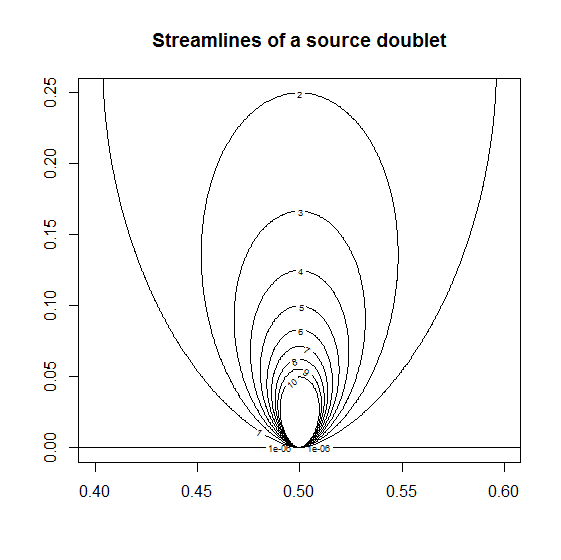
\includegraphics[scale=.5]{c2f2}}
\caption{Streamlines in an axial plane}
\label{c2f2}
\end{figure}

It was generated using the following R code.
\begin{verbatim}
# To draw the stream lines as in the textbook, 
# interchange x and z axes. The diagram is 
# drawn in XZ plane.

z <- seq(from = -2, to = 2, len = 1000)
x <- seq(from = 1e-6, to = 2, len = 1000)

f <- function(x, z) {
	x^2/(x^2 + z^2)^(3/2)
}

psi <- outer(x, z, FUN = 'f')

# Values of level curves
lv <- c(1e-6, 1, 2, 3, 4, 5, 6, 7, 8, 9, 10) 

# To draw the contours with z axis set 
# horizontally, we transpose the psi.
Xl <- c(0.4, 0.6)
Yl <- c(0.0, 0.25)
contour(t(psi), levels = lv, xlim = Xl, ylim = Yl)
title('Streamlines of a source doublet')
\end{verbatim}
A few points to note:
\begin{itemize}
\item We don't have to plot $\vec{u}_e$. Plotting $\psi$ suffices to get a visual impression of the flow.
\item The plot of streamlines does not give us the direction of the flow. For an axisymmetric flow, as this one, the velocity in spherical polar coordinates is given by equation (2.2.14)
as
\[
\vec{u}_e = \frac{1}{s^2\sin\theta}\pdt{\psi}{\theta}\uvec{s} - \frac{1}{s\sin\theta}\pdt{\psi}{s}\uvec{\theta},
\]
where for sake of consistency, we have used $s$ instead of $r$.
\item The source doublet at $\vec{x}^\op$ comprised of a point source of strength $m$ at $\vec{x}^\op + \delta\vec{x}^\op/2$ and a sink of strength $-m$ at 
$\vec{x}^\op - \delta\vec{x}^\op/2$. Thus, the direction of $\vec{\mu}$ is along the positive $z$ axis, shown horizontal in figure \ref{c2f2}. Therefore, the direction of the velocity
will be anti-clockwise along the streamlines.
\end{itemize}

\item Now let us consider a source doublet of strength $\vec{\mu}$ placed at $\vec{x}^\op + \delta\vec{x}^\op/2$ and that of strength $-\vec{\mu}$ placed at 
$\vec{x}^\op - \delta\vec{x}^\op/2$. The potential due to them is
\[
\phi_e(\vec{x}) = \frac{\vec{\mu}}{4\pi}\cdot\grad{\left(\frac{1}{\vec{x} - \vec{x}^\op - \delta\vec{x}^\op/2}\right)} - 
 \frac{\vec{\mu}}{4\pi}\cdot\grad{\left(\frac{1}{\vec{x} - \vec{x}^\op + \delta\vec{x}^\op/2}\right)}
\]
which, in Cartesian tensor notation, and some simplification gives,
\[
\phi_e(\vec{x}) = \frac{\mu_i}{4\pi}\frac{\partial}{\partial x_i}\left(\frac{1}{\vec{s} - \delta\vec{x}^\op/2} - \frac{1}{\vec{s} + \delta\vec{x}^\op/2}\right)
\]
which is,
\[
\phi_e(\vec{x}) = \frac{\mu_i}{4\pi}\frac{\partial}{\partial x_i}\frac{\vec{s}\cdot\delta\vec{x}^\op}{s^3} = \frac{\mu_i}{4\pi}\frac{\partial}{\partial x_i}\frac{s_j\delta x_j}{s^3}
\]
Let $\nu_{ij} = \mu_i \delta x_j$. Using the fact that
\[
\grad{\left(\frac{1}{s}\right)} = -\frac{\vec{s}}{s^3}
\]
we get
\[
\phi_e(\vec{x}) = -\frac{\nu_{ij}}{4\pi}\frac{\partial^2}{\partial x_i \partial x_j}\left(\frac{1}{s}\right)
\]
This expression is analogous to the potential at $\vec{x}$ due to an electric quadrupole at $\vec{x}^\op$. The quadrupole moment tensor is $\nu_{ij}$.

\item There is another way to get equations (2.5.7) and (2.5.8) of the book. Consider an infinite line of point sources with density $m$. Without loss of generality, we can make the $z$ 
axis coincide it. We want to find the velocity at a point $(x, y, 0)$ on the $XY$ plane. Consider a cylindrical surface with axis along the $z$ axis and passing through $(x, y, 0)$. Let 
it have a length $L$.=such that the $z$ coordinate ranges from $-L/2$ to $L/2$. Integrate $\dive{\vec{u}_e} = \Delta$ over the volume of this imaginary surface. Thus,
\[
\int\dive{\vec{u}_e}\un dV = \int\Delta dV
\]
or, since $\Delta = m\delta(x)\delta(y)$,
\[
\int\vec{u}_e\cdot\un dA = \int m\delta(x)\delta(y) dx dy dz = \int_{-L/2}^{L/2} mdz = mL
\]
Since $\vec{u}_e$ is only in the radial direction, the surface integral on the left hand side across the upper and lower surfaces is zero. (The unit vector $\un$ on these surfaces is
perpendicular to $\vec{u}_e$.) On the curved surface, $\vec{u}_e$ and $\un$ are parallel to each other and hence,
\[
u_e 2\pi\sigma L = mL
\]
or that 
\[
u_e = \frac{m}{2\pi} \frac{1}{\sigma}
\]
or, remembering that $\vec{u}_e$ is along the radial direction,
\[
\vec{u}_e = u_e \uvec{\sigma} = u_r \frac{\vec{\sigma}}{\sigma} = u_e \frac{x\uvec{x} + y\uvec{y}}{\sqrt{x^2 + y^2}} = \frac{x\uvec{x} + y\uvec{y}}{\sigma}
\]
or
\[
\vec{u}_e = \frac{m}{2\pi} \left(\frac{x}{\sigma}\uvec{x} + \frac{y}{\sigma}\uvec{y}\right)
\]
Since $\vec{u}_e = \grad{\phi}$ and if the point $A$ is a \enquote*{reference point} for the potential then,
\[
\int_A^{\sigma} \vec{u}_e\cdot d\vec{x}^\op = \int_A^{\sigma} \grad{\phi}\cdot d\vec{x}^\op
\]
or
\[
\frac{m}{2\pi} \ln\sigma - \frac{m}{2\pi} \ln\sigma_A = \phi(\sigma) - \phi(\sigma_A)
\]
This technique is similar to that of finding electric field due to an infinite line of charges, distributed uniformly.
\end{itemize}

\section{The vorticity distribution}\label{c2s6}
\begin{itemize}
\item Unlike the velocity field, the vorticity is always solenoidal. A vortex line is an imaginary line in the fluid which is always tangential to the vorticity field. If $d\vec{x}$ is 
a small element of the vortex line, then because it is always tangential to $\vec{\omega}$, $\vec{\omega} \vp d\vec{x} = 0$. That is,
\[
\uvec{x}(\omega_y dz - \omega_z dy) + \uvec{y}(\omega_z dx - \omega_x dz) + \uvec{z}(\omega_x dy - \omega_y dx) = 0
\]
or
\[
\frac{dx}{\omega_x} = \frac{dy}{\omega_y} = \frac{dz}{\omega_z}
\]
is the equation of the vortex lines. A surface in the fluid formed by all vortex lines passing through an irreducible curve in the fluid is called a vortex tube. 

\item A vortex tube cannot end in the interior of the fluid. For if it did, then if $C$ is the curve at the end of the vortex tube and $A$ is the area enclosed by it,
\[
\int_A \vec{\omega}\cdot\un dA = 0
\]
Let $C^\op$ be a curve which coincides with the cross section of the vortex tube, a little behind its end. Let $A^\op$ is the area enclosed by it. Let $S$ be the curved area between
$C^\op$ and $C$. Then, if $V$ is the volume bound by $A$, $A^\op$ and $S$,
\[
\int_V \dive{\vec{\omega}} dV = \int_{A} \vec{\omega}\cdot\un dA + \int_{S} \vec{\omega}\cdot\un dA + \int_{A^\op} \vec{\omega}\cdot\un dA
\]
Of the three integrals on the right hand side of the above equation, the first one is zero because the vortex tube ends there, the second one is zero because the surface is tangential
to the vorticity field and the third one is non-zero. Therefore,
\[
\int_V \dive{\vec{\omega}} dV \ne 0
\]
violating the fact that $\vec{\omega}$ is always solenoidal.

\item An immediate consequence of the above point is that vortex lines are closed curves. (The way lines of magnetic field are closed curves.)

\item It is also true that 
\[
\int_A \vec{\omega}\cdot\un dA 
\]
is the same across all cross sections of a vortex tube. It is thus a characteristic of the vortex tube and is called the strength of the tube.

\item Let $A$ be an open surface inside a fluid, bound by a closed curve $C$. The quantity,
\[
\int\vec{\omega}\cdot\un dA = \oint_C \vec{u}\cdot d\vec{x},
\]
is called the circulation round $C$.

\item Consider a flow in which the vorticity is quite high only in the neighborhood of a line. Consider a vortex tube enclosing the line. Shrink its cross section such that as its cross 
section goes to zero, the integral
\[
\int_A \vec{\omega}\cdot\un dA 
\]
remains constant, say $\kappa$. Such a singularity is called a vortex line. Since
\[
\int_A \vec{\omega}\cdot\un dA = \kappa,
\]
if $\delta\vec{l}$ is a line element along the line vortex,
\[
\delta\vec{l}\int_A \vec{\omega}\cdot\un dA = \kappa\delta\vec{l},
\]
But $\delta\vec{l}\cdot\un dA = dV$ and hence,
\[
\int_{\delta V} \vec{\omega} dV = \kappa\delta\vec{l}
\]
That is, for a small volume element, $\vec{\omega}\delta V = \kappa\delta\vec{l}$. Since
\[
\vec{u}_v = -\frac{1}{4\pi}\int\frac{\vec{s} \vp \vec{\omega}(\vec{x}^\op)}{s^3} dV(\vec{x}^\op),
\]
for a vortex line of strength $\kappa$, we have
\begin{equation}\label{c2s6e1}
\vec{u}_v = -\frac{\kappa}{4\pi}\int \frac{\vec{s} \vp d\vec{l}(\vec{x}^\op)}{s^3}
\end{equation}

\item Consider an infinitely long line vortex of strength $\kappa$. Referring to figure 2.6.1 of the book, it is clear that $s^2 = \sigma^2 + l^2$, $l$ being measured along the line
vortex. If $\theta$ is the angle between $d\vec{l}$ and $\vec{s}$,
\[
|\vec{s} \vp d\vec{l}| = sdl\sin\theta = sdl\sin(\pi - \theta) = sdl\frac{\sigma}{s} = \sigma dl
\]
and hence,
\[
|\vec{u}_v| = \frac{\kappa}{4\pi}\int_{-\infty}^\infty \frac{\sigma}{(\sigma^2 + l^2)^{3/2}} dl
\]
Put $l = \sigma\tan\alpha$, so that
\begin{eqnarray*}
\int_{-\infty}^\infty \frac{\sigma}{(\sigma^2 + l^2)^{3/2}} dl &=& \int_{-\pi/2}^{\pi/2} \frac{\sigma^2\sec^2\alpha}{\sigma^3\sec^3\alpha} d\alpha \\
 &=& \frac{1}{\sigma}\int_{-\pi/2}^{\pi/2}\cos\alpha d\alpha \\
 &=& \frac{2}{\sigma}
\end{eqnarray*}
so that
\[
|\vec{u}_v| = \frac{\kappa}{2\pi\sigma}
\]
Further, the direction of $\vec{u}_v$ is along $\uvec{\phi}$ (of cylindrical coordinate system). Therefore, from (2.2.10) of the book,
\[
\frac{\kappa}{2\pi\sigma} = -\pdt{\psi}{\sigma}
\]
or that
\[
\sigma = -\frac{\kappa}{2\pi}\ln\sigma
\]

\item Since
\[
\grad{\left(\frac{1}{s}\right)} = -\frac{\vec{s}}{s^3},
\]
we have from \eqref{c2s6e1},
\[
\vec{u}_v = \frac{\kappa}{4\pi}\int \grad{\left(\frac{1}{s}\right)} \vp d\vec{l}(\vec{x}^\op)
\]
Further, since $\curl{(\psi\vec{A})} = \psi\curl{\vec{A}} + \grad{\psi}\vp\vec{A}$,
\[
\curl{\left(\frac{d\vec{l}(\vec{x}^\op)}{s}\right)} = \grad{\left(\frac{1}{s}\right)} \vp d\vec{l}(\vec{x}^\op)
\]
so that,
\[
\vec{u}_v = \frac{\kappa}{4\pi} \int \curl{\left(\frac{d\vec{l}(\vec{x}^\op)}{s}\right)} = \curl\int \frac{\kappa d\vec{l}(\vec{x}^\op)}{4\pi s}
\]
Using \eqref{c2sae6},
\[
\int \frac{\kappa d\vec{l}(\vec{x}^\op)}{4\pi s} = -\frac{\kappa}{4\pi}\int\nabla^\op\left(\frac{1}{s}\right)\vp\un dA(\vec{x}^\op)
\]
or,
\[
\vec{u}_v = -\frac{\kappa}{4\pi} \curl \int\nabla^\op\left(\frac{1}{s}\right)\vp\un dA(\vec{x}^\op) = 
-\frac{\kappa}{4\pi}\int\curl{\left(\nabla^\op\left(\frac{1}{s}\right)\vp\un\right)} dA(\vec{x}^\op)
\]
Now, since $\un$ depends only on $\vec{x}^\op$,
\[
\curl{\left(\nabla^\op\left(\frac{1}{s}\right)\vp\un\right)} = \un\dive{\nabla^\op\left(\frac{1}{s}\right)} + (\un\cdot\nabla)\nabla^\op\left(\frac{1}{s}\right)
\]
Further,
\[
\dive{\nabla^\op\left(\frac{1}{s}\right)} = -\dive{\grad{\left(\frac{1}{s}\right)}} = -\nabla^2\left(\frac{1}{s}\right) = 0,
\]
because $1/s$ is a solution of Laplace's equation in three dimensions. Thus,
\[
\curl{\left(\nabla^\op\left(\frac{1}{s}\right)\vp\un\right)} = (\un\cdot\nabla)\nabla^\op\left(\frac{1}{s}\right)
\]
and hence,
\[
\vec{u}_v = -\frac{\kappa}{4\pi} \int (\un\cdot\nabla)\nabla^\op\left(\frac{1}{s}\right)dA(\vec{x}^\op)
\]
Since,
\[
\grad{\left(\frac{1}{s}\right)} = -\frac{\vec{s}}{s^3} = -\nabla^\op\left(\frac{1}{s}\right)
\]
we have,
\[
\vec{u}_v = -\frac{\kappa}{4\pi} \int \un \cdot \nabla \frac{\vec{s}}{s^3} dA(\vec{x}^\op)
\]
Since $\un$ depends only on $\vec{x}^\op$,
\[
\grad{\left(\un\cdot\frac{\vec{c}}{s^3}\right)} = \un \cdot \nabla \frac{\vec{s}}{s^3} + \un \vp \curl{\frac{\vec{s}}{s^3}}
\]
But,
\[
\frac{\vec{s}}{s^3} = -\grad{\left(\frac{1}{s}\right)}
\]
therefore its curl vanishes and hence,
\[
\grad{\left(\un\cdot\frac{\vec{s}}{s^3}\right)} = \un \cdot \nabla \frac{\vec{s}}{s^3}
\]
so that,
\[
\vec{u}_v = -\frac{\kappa}{4\pi} \int \grad{\left(\un\cdot\frac{\vec{s}}{s^3}\right)} dA(\vec{x}^\op)
\]
or,
\[
\vec{u}_v = -\frac{\kappa}{4\pi} \grad{\int \left(\frac{\un\cdot\vec{s}}{s^3}\right) dA(\vec{x}^\op)}
\]
The line vortex is a closed curve and it subtends a solid angle $\Omega$ at the point $\vec{x}$, as shown in figure \ref{c2f3}.
\begin{figure}[!ht]
\centering
\centerline{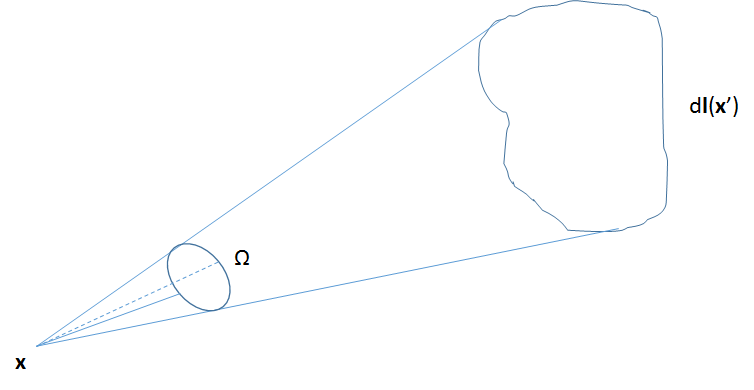
\includegraphics[scale=.5]{c2f3}}
\caption{Solid angle subtended by a line vortex}
\label{c2f3}
\end{figure}
Thus,
\[
\Omega(\vec{x}) = \int \left(\frac{\un\cdot\vec{s}}{s^3}\right) dA(\vec{x}^\op)
\]
so that,
\[
\vec{u}_v = -\frac{\kappa}{4\pi} \grad{\Omega(\vec{x})}
\]

\item Equation (2.6.5) of the book gives stream function for a line vortex of strength $\kappa$ as
\[
\psi = -\frac{\kappa}{2\pi}\ln\sigma,
\]
where $\sigma^2 = (x - x^\op)^2 + (y - y^\op)^2$. In a vortex doublet, two line vortices of strengths of opposite signs are close to each other. If a line vortex of strength 
$\kappa$ is at $\vec{x}^\op + \delta\vec{x}^\op/2$ then its stream function is
\[
\psi_{+} = -\frac{\kappa}{2\pi}f(\vec{x}; \vec{x}^\op + \delta\vec{x}^\op/2),
\]
where 
\[
f(\vec{x}; \vec{x}^\op) = \ln\sigma
\]
Similarly, a line vortex of strength $-\kappa$ at $\vec{x}^\op - \delta\vec{x}^\op$ has a stream function,
\[
\psi_{-} = -\frac{\kappa}{2\pi}f(\vec{x}; \vec{x}^\op - \delta\vec{x}^\op/2),
\]
If $\vec{u}_1$ is associated with a vector potential $\vec{B}_1 = (0, 0, \psi_1)$ and $\vec{u}_2$ is associated with $\vec{B}_2 = (0, 0, \psi_2)$ , then it is clear that if $\vec{u}
= \vec{u}_1 + \vec{u}_2$ then since
\[
\vec{u} = \curl{\vec{B}_1} + \curl{\vec{B}_2} = \curl{(\vec{B}_1 + \vec{B}_2)},
\]
the vector potential associated with $\vec{u}$ is $\curl{(\vec{B}_1 + \vec{B}_2)} = (0, 0, \psi_1 + \psi_2)$. Therefore, the stream function of vortex doublet is
\[
\psi = \psi_1 + \psi_2 = 
-\frac{\kappa}{2\pi}\left(f\left(\vec{x}; \vec{x}^\op + \frac{\delta\vec{x}^\op}{2}\right) - f\left(\vec{x}; \vec{x}^\op - \frac{\delta\vec{x}^\op}{2}\right)\right)
\]
Expanding $f$ as a Taylor series and retaining the first order terms, we get
\[
\psi = -\frac{\kappa}{2\pi}\delta\vec{x}^\op\cdot\nabla^\op{f} = \frac{\kappa}{2\pi}\frac{\delta\vec{x}^\op\cdot\vec{s}}{\sigma^2}
\]
If 
\[
\vec{\lambda} = \lim_{\delta\vec{x}^\op \rightarrow 0} \kappa\delta\vec{x}^\op
\]
then
\[
\psi = \frac{1}{2\pi}\frac{\vec{\lambda}\cdot\vec{s}}{\sigma^2}
\]

\item If we now want to plot the stream function, we assume that the vortex doublet of unit strength $2\pi$ is aligned along the $x$-axis. That is, $\vec{\lambda} = 2\pi\uvec{x}$. 
If we also assume that the vortex doublet is at the origin then $(x^\op, y^\op) = (0, 0)$. Therefore, in Cartesian coordinates, the stream function is
\[
\psi = \frac{1}{2\pi}\frac{2\pi x}{x^2 + y^2}
\]
Figure \ref{c2f4} shows the stream lines.
\begin{figure}[!ht]
\centering
\centerline{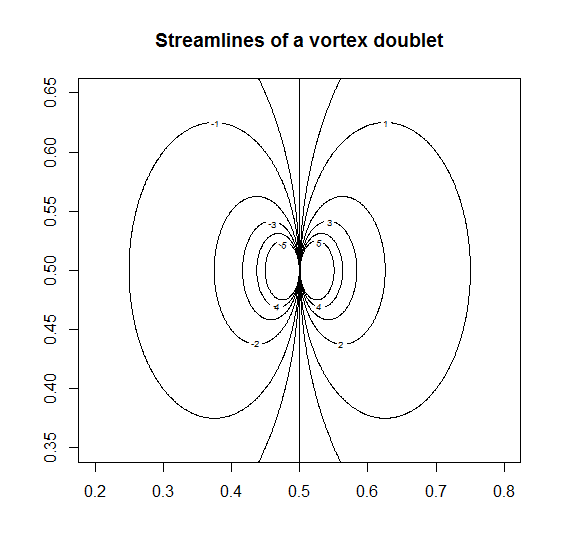
\includegraphics[scale=.5]{c2f4}}
\caption{Streamlines due to a vortex doublet}
\label{c2f4}
\end{figure}

It was generated using the following R code.
\begin{verbatim}
# To draw the stream lines as in the textbook, 
# interchange x and z axes. The diagram is 
# drawn in XZ plane.
y <- seq(from = -2, to = 2, len = 1000)
x.pos <- seq(from = 1e-6, to = 2, len = 500)
x.neg <- seq(from = -2, to = -1e-6, len = 500)
x <- c(x.neg, x.pos)

f <- function(x, y) {
	(x)/(x^2 + y^2)
}

psi <- outer(x, y, FUN = 'f')

# Values of level curves
lv <- c(-5, -4, -3, -2, -1, 1e-6, 1, 2, 3, 4, 5) 

# To draw the contours with z axis set 
# horizontally, we transpose the psi.
Xl <- c(0.2, 0.8)
Yl <- c(0.35, 0.65)
contour(psi, levels = lv, xlim = Xl, ylim = Yl)
title('Streamlines of a vortex doublet'))
\end{verbatim}

Since the vortex doublet consisted of vortex of strength $+\kappa$ at $\vec{x}^\op + \delta\vec{x}^\op/2$ and another one of $-\kappa$ at $\vec{x}^\op - \delta\vec{x}^\op/2$, the stream
lines on the right have an anti-clockwise direction and those on the left have a clockwise direction.

\item Sometimes there is a considerable concentration of vorticity on a surface in a fluid. It shows up as a large collection of line vortices, all lying on the surface. We define the 
strength density of such a vortex sheet by
\[
\vec{\Gamma} = \int\vec{\omega}dx_n,
\]
where $x_n$ is the distance normal to the surface and the integral is over a small range $\epsilon$ containing the surface. We assume that as $\epsilon \rightarrow 0$, the integral
remains constant so that $\vec{\Gamma}$ is a local characteristic of the vortex sheet. Recall that the strength of a vortex tube is defined as 
\[
\kappa = \int\vec{\omega}\cdot\un dA,
\]
where $\un$ is a unit vector normal to the cross section of the tube over which we are evaluating the surface integral. In particular, it is \emph{not} a normal to the vortex sheet. It
is in fact, in the vortex sheet. We can write it as
\[
\kappa = \iint\vec{\omega}\cdot\un dx dy \approx \int\vec{\omega}dx \cdot \un \left(\delta y\right) = \left(\vec{\Gamma}\cdot\un\right)\delta y,
\]
or $\vec{\Gamma}\cdot\un$ is the strength of the vortex tube \emph{per unit width} of the tube. Refer to figure \ref{c2f5} for a diagram of the vortex sheet and the tubes it contains.
\begin{figure}[!ht]
\centering
\centerline{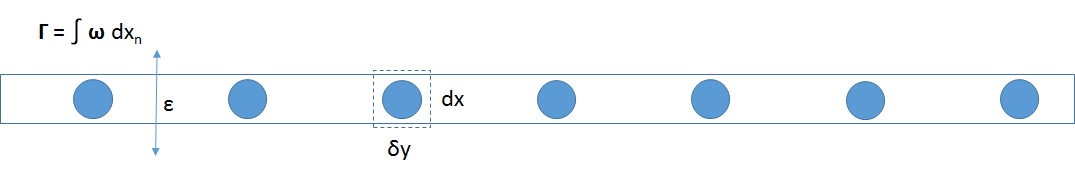
\includegraphics[scale=.35]{c2f5}}
\caption{Sheet vortex}
\label{c2f5}
\end{figure}
The rectangle depicts the vortex sheet and the blue circles denote the vortex tubes. The arrow across the sheet depicts the range of integration in the definition of $\vec{\Gamma}$. The
vorticity $\vec{\omega}$ and the strength density of the vortex sheet $\vec{\Gamma}$ are parallel to each other and perpendicular to the plane of the diagram.

\item The idea of considering $\epsilon \rightarrow 0$ is equivalent to considering the vortex sheet to be infinite in extent. We will use this interpretation in the next point.

\item Let us now consider the velocity \enquote*{due to} a vortex sheet. Equation (2.4.11) of the book is
\[
\vec{u}_v = -\frac{1}{4\pi}\int\frac{\vec{s}\vp\vec{\omega}(\vec{x}^\op)}{s^3} dV(\vec{x}^\op)
\]
If most of the vorticity is concentrated in a vortex sheet, we can approximate $\vec{\omega} dV(\vec{x}^\op)$ by $\vec{\Gamma} dA(\vec{x}^\op)$ so that
\[
\vec{u}_v = -\frac{1}{4\pi}\int\frac{\vec{s}\vp\vec{\Gamma}(\vec{x}^\op)}{s^3} dA(\vec{x}^\op)
\]
In the case of a single plane sheet vortex on which $\vec{\Gamma}$ is uniform,
\[
\vec{u}_v = \frac{\vec{\Gamma}}{4\pi}\vp\int\frac{\vec{s}}{s^3} dA(\vec{x}^\op)
\]
Close to the sheet, the plane can be considered to be infinitely large and yet having a uniform $\vec{\Gamma}$. In such a situation, we can write $\vec{s}$ as a sum of two vectors,
one parallel to $\vec{\Gamma}$ and the other parallel to $\un$. If $\uvec{\Gamma}$ is a unit vector parallel to $\vec{\Gamma}$ then,
\[
\vec{s} = (\vec{s}\cdot\uvec{\Gamma})\uvec{\Gamma} + (\vec{s}\cdot\un)\un
\]
so that
\[
\vec{\Gamma} \vp \vec{s} = \vec{\Gamma} \vp (\vec{s}\cdot\un)\un
\]
and hence,
\[
\vec{u}_v = \frac{\vec{\Gamma}}{4\pi}\vp\int\frac{\vec{s}\cdot\un}{s^3}\un dA(\vec{x}^\op)
\]
We can write the integral as,
\[
\vec{u}_v = \frac{\vec{\Gamma}}{4\pi}\vp\un \int d\Omega,
\]
where $\Omega$ denotes the solid angle subtended by the sheet vortex at $\vec{x}$. Since we are integrating only over the \enquote{below} $\vec{x}$, the value of the integral is half
of the total solid angle so that,
\[
\vec{u}_v = \frac{\vec{\Gamma}}{4\pi}\vp\un 2\pi = \frac{1}{2}\vec{\Gamma}\vp\un
\]
If $\vec{\Gamma}$ is perpendicular to the plane of figure \ref{c2f6} and pointing outwards, the velocity just above and just below the plane are equal and opposite to each other.
\begin{figure}[!ht]
\centering
\centerline{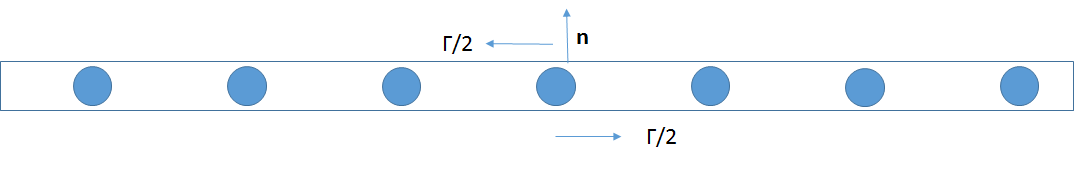
\includegraphics[scale=.35]{c2f6}}
\caption{Velocity around a sheet vortex}
\label{c2f6}
\end{figure}

\item Now consider a sheet vortex in the form of a cylinder of arbitrary cross section. The generators of the cylinder are lines along the curved surface of the cylinder, connecting its
cross sections. Let $\vec{\Gamma}$ be always perpendicular to the generators and of the same magnitude all over. Equation (2.6.8) of the book is
\[
\vec{u}_v(\vec{x}) = -\frac{1}{4\pi}\int\frac{\vec{s}\vp\vec{\Gamma}(\vec{x}^\op)}{s^3} dA(\vec{x}^\op)
\]
Consider a point $\vec{x}^\op$ on the surface of the cylinder. Let $d\vec{l}(\vec{x}^\op)$ be a line element in the direction of $\vec{\Gamma}$ and $dm(\vec{x}^\op)$ be a line 
element perpendicular to $\vec{\Gamma}$. Then, $\vec{\Gamma}(\vec{x}^\op) dA(\vec{x}^\op) = \vec{\Gamma}(\vec{x}^\op) dl(\vec{x}^\op) dm(\vec{x}^\op) = 
\Gamma d\vec{l}(\vec{x}^\op)dm(\vec{x}^\op)$ so that
\[
\vec{u}_v(\vec{x}) = -\frac{\Gamma}{4\pi}\int_{-\infty}^\infty \oint \frac{\vec{s}\vp d\vec{l}(\vec{x}^\op)}{s^3} dm(\vec{x}^\op),
\]
where the first integral is over $m$ and the second one over $\vec{l}$. Interchanging the order of integration,
\[
\vec{u}_v(\vec{x}) = -\frac{\Gamma}{4\pi} \oint \int_{-\infty}^\infty \frac{\vec{s}dm(\vec{x}^\op)}{s^3} \vp d\vec{l}(\vec{x}^\op),
\]
Write $\vec{s} = \vec{p} + \vec{m}$, where $\vec{p}$ is in the cross sectional plane while $\vec{m}$ is perpendicular to it. Further, let $\uvec{p}$ and $\uvec{m}$ be the unit 
vectors along $\vec{p}$ and $\vec{m}$ so that,
\[
\int_{-\infty}^{\infty} \frac{\vec{s}}{s^3}dm = \uvec{p}\int_{-\infty}^{\infty} \frac{p}{(p^2 + m^2)^{3/2}} dm + \uvec{m}\int_{-\infty}^{\infty} \frac{m}{(p^2 + m^2)^{3/2}} dm
\]
Let the right hand side be written as $\uvec{p}I_1 + \uvec{m}I_2$. In $I_1$, put $m = p\tan\alpha$ so that
\[
I_1 = \int_{-\pi/2}^{\pi/2} \frac{p^2\sec^2\alpha}{p^3\sec^3\alpha} d\alpha = \frac{1}{p}\int_{-\pi/2}^{\pi/2}\cos\alpha d\alpha = \frac{2}{p}
\]
In $I_2$, put $n^2 = m^2 + p^2$ so that
\[
I_2 = \int_{-\infty}^{\infty} \frac{ndn}{n^3} = 0
\]
and hence
\[
\int_{-\infty}^{\infty} \frac{\vec{s}}{s^3}dm = \uvec{p}\frac{2}{p} = \frac{2\vec{p}}{p^2}
\]
We now have,
\[
\vec{u}_v(\vec{x}) = -\frac{\Gamma}{2\pi}\oint\frac{\vec{p} \vp d\vec{l}(\vec{x}^\op)}{p^2}
\]

\item We will now argue that
\[
\oint\frac{\vec{p} \vp d\vec{l}(\vec{x}^\op)}{p^2}
\]
is zero if the observation point $\vec{x}$ is outside the cylinder and $2\pi$ if it is inside. For a point $\vec{x}$ that is inside the cylinder, we can write $d\vec{l}(\vec{x}^\op) = 
pd\theta$ so that
\[
\oint\frac{\vec{p} \vp d\vec{l}(\vec{x}^\op)}{p^2} = \int_0^{2\pi} \uvec{a} d\theta = 2\pi\uvec{a},
\]
where $\uvec{a}$ is perpendicular to both $\vec{p}$ and $d\vec{l}(\vec{x}^\op)$, which means that it is parallel to the axis of the cylinder. Now consider a point $\vec{x}$ that is
outside the cylinder. Referring to figure \ref{c2f7}, let the angle between $\vec{p}$ and $d\vec{l}(\vec{x}^\op)$ span from $\pi/2 - \theta$ (at point $A$) to $\pi/2 + \theta$ (at point 
$C$). The angle keeps on increasing from $\pi/2 + \theta$ at $C$ to $3\pi/2$ at $D$ and $2\pi + \pi/2 - \theta = \pi/2 - \theta$ at $A$. Therefore,
\[
\oint\frac{\vec{p} \vp d\vec{l}(\vec{x}^\op)}{p^2} = \int_{\pi/2 - \theta}^{\pi/2 + \theta}\uvec{b}d\theta + \int_{\pi/2 + \theta}^{\pi/2 - \theta}\uvec{b}{p}d\theta = 0
\]
where $\uvec{b}$ is a unit vector in the direction of $\vec{p} \vp d\vec{l}(\vec{x}^\op)$. The key to this proof is the independence of the integrand from $p$. Writing $dl = pd\theta$
cancels the second power of $p$ in the denominator, the first power being cancelled by $\vec{p}$\footnote{This result is similar to the one in electrodynamics where the magnetic field 
outside a solenoid is zero while inside it is parallel to the axis}.
\begin{figure}[!ht]
\centering
\centerline{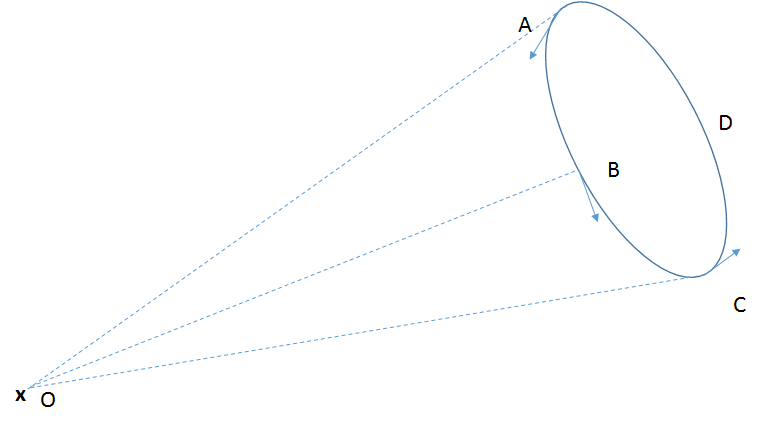
\includegraphics[scale=.35]{c2f7}}
\caption{Integration when the field point is outside the cylinder}
\label{c2f7}
\end{figure}

\item In order to prove that the component of $\vec{u}_v$ normal to the sheet vortex is continuous across the sheet, we consider a \enquote*{gaussian pillbox} as shown in figure 
\ref{c2f8}. Let $\vec{u}_v = \vec{u}_p + \vec{u}_n$, where $\vec{u}_p$ is the component of velocity in the plane of the sheet vortex and $\vec{u}_n$ is the component normal to it. 
Integrating $\dive{\vec{u}_v}$ over the pillbox,
\[
\int\dive{\vec{u}_v}dV = \oint\vec{u}_v\cdot\un dA.
\]
If the pillbox is shrunk so that its height is very small, for an incompressible fluid,
\[
0 = \int_{U} \vec{u}_v^{u} dA - \int_{L} \vec{u}_v^{l} dA,
\]
where $U$ and $L$ are the upper and lower plane surfaces of the pillbox. Since their areas are identical,
\[
\int_U (\vec{u}_v^{u} - \vec{u}_v^{l})dA = 0,
\]
or that the normal component of $\vec{u}_v$ is continuous across the sheet.
\begin{figure}[!ht]
\centering
\centerline{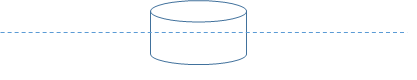
\includegraphics[scale=0.9]{c2f8}}
\caption{A gaussian pillbox straddling the sheet vortex}
\label{c2f8}
\end{figure}
\end{itemize}

\section{Irrotational and solenoidal velocity distributions}\label{c2s7}
\begin{itemize}
\item Most fluids behave, under a wide range of flow conditions, as if they were nearly incompressible. Further, over large parts of the velocity field, the vorticity is indeed zero.
Therefore, it is useful to study fields $\vec{v}$ that satisfy $\dive{\vec{v}} = 0$ and $\curl{\vec{v}} = 0$. Such a fluid element does not undergo a change in volume, nor does it have
a local rotation. The second of the above equations suggests that we can find a scalar function $\phi(\vec{x})$ such that $\vec{v} = \grad{\phi}$, which put in the first equation gives
\[
\nabla^2\phi = 0,
\]
or that $\phi$ is a harmonic function. Solutions of Laplace's equations are smooth, with all derivatives remaining smooth throughout the domain, except possibly at the boundary points. (
This is in contrast with the hyperbolic equations whose solutions may have discontinuities in the form of shocks.)

\item Figure 2.7.1, to my eyes, is a multiply connected region and is identical to fig. 2.8.1. If we have to interpret it as a singly connected region, then we assume that there is no
inner boundary for finite flows and no outer boundary in the case of infinite flows.

\item Let us consider only finite flows. Since $\vec{v} = \grad{\phi}$,
\[
\dive{(\phi\vec{v})} = \phi\dive{\vec{v}} + \vec{v}\cdot\grad{\phi} = 0 + v^2,
\]
so that
\[
\int v^2 dV = \int\dive{(\phi\vec{v})}dV = \int \phi\vec{v}\cdot\un dA
\]
If the normal component of the velocity on the boundary of the volume is zero, then the integrand on the right hand side is zero so that 
\begin{equation}\label{c2s7e1}
\int v^2 dV = 0,
\end{equation}
which, for real values of $\vec{v}$ implies $\vec{v} = 0$ throughout the volume. Similar analysis works for infinite flows, where we do not have the outer boundary.

\item If $\phi_1$ and $\phi_2$ are two solutions of $\nabla^2\phi = 0$ then so is $\phi = \phi_1 - \phi_2$. Let $\vec{v} = \grad{\phi}, \vec{v}_1 = \grad{\phi}_1$ and 
$\vec{v}_2 = \grad{\phi}_2$. Equation \eqref{c2s7e1}, applied to $\vec{v}$ gives $\vec{v} = 0$ or that $\vec{v}_1 = \vec{v}_2$ if $(\vec{v}_1 - \vec{v}_2)\cdot\un = 0$ on the boundary.

\item An often used mathematical idealization is that of a fluid of an infinite extent. When we use it, the inner boundary in figure 2.7.1 comes into play and the outer one does not. It
will be shown later that one of the conditions for having a unique solution to $\nabla^2\phi = 0$ is that the normal component of $\vec{v}$ take a prescribed value on the inner boundary.

\item Recall that the velocity of the fluid is $\vec{u} = \vec{u}_e + \vec{u}_v + \vec{v}$, where $\vec{u}_e$ is due to a given rate of expansion, $\vec{u}_v$ is due to a given vorticity
and $\vec{v}$ is what is needed to satisfy boundary conditions. It is the last component that is irrotational and solenoidal and therefore described by the velocity potential $\phi$. 
Further, the boundary conditions must be prescribed in terms of $\vec{v}$ and \emph{not} $\vec{u}$.

\item An example of a fluid of infinite extent and having the internal boundary is when a rigid body (of size small in comparison of the extent of the fluid) moves through a fluid 
otherwise at rest. If the body moves with a velocity $\vec{U}$ then the normal component of $\vec{v}$ is
\[
\vec{U}\cdot\un - (\vec{u}_e + \vec{u}_v)\cdot\un
\]
Neither the body's acceleration nor its past history determines the motion of the fluid, only its instantaneous velocity $\vec{U}$ matters.

\item Consider a two dimensional, irrotational and solenoidal field. If $\vec{v} = \grad{\phi}$ and if $v_x = kx$ and $v_y = ly$ then $\dive{\vec{v}} = 0$ gives $l = -k$. The relation
$v_x = \partial\phi/\partial x$ gives $\phi(x, y) = kx^2/2 + f_1(y)$. Similarly, $v_y = \partial\phi/\partial y$ gives $\phi(x, y) = -ky^2/2 + f_2(x)$. The two expressions for $\phi$
imply that $\phi(x, y) = k(x^2 - y^2)/2 + c_1$, where $c_1$ is a constant. If $\psi$ is the stream function corresponding to $\vec{v}$ then $\vec{v} = \curl{\vec{B}}$, where 
$\vec{B} = (0, 0, \psi)$. That is,
\begin{eqnarray*}
v_x &=& \pdt{\psi}{y} \\
v_y &=& -\pdt{\psi}{x}
\end{eqnarray*}
The first of the above equations gives $\psi(x, y) = kxy + g_1(x)$ while the second one gives $\psi(x, y) = kxy + g_2(y)$. The two together give $\psi(x, y) = kxy + c_2$, where $c_2$ is
another constant. Both $\phi$ and $\psi$ are equations of rectangular hyperbolae.

\item If we repeat the analysis of the previous point now for a axisymmetric flow described in a cylindrical coordinate system, 
\[
\dive{\vec{v}} = \pdt{v_x}{x} + \frac{1}{\sigma}\pdt{(\sigma v_\sigma)}{\sigma}
\]
If $v_x = kx$ and $v_\sigma = l\sigma$ then
\[
\dive{\vec{v}} = k + \frac{1}{\sigma}2l\sigma 
\]
so that $\dive{\vec{v}} = 0 \Rightarrow l = -k/2$. $v_x = \partial\phi/\partial x$ gives $\phi(x, \sigma) = kx^2/2 + f_1(\sigma)$, while $v_\sigma = \partial\phi/\partial\phi$ gives
$\phi(x, \sigma) = -k\sigma^2/4 + f_2(x)$. The two together give 
\[
\phi(x, y) = \frac{k}{2}\left(x^2 - \frac{\sigma^2}{2}\right)
\]
We can always replace the constant $k/2$ by another one, $k$. The equations for stream function (refer to (2.2.11) in the book) are
\begin{eqnarray*}
v_x &=& \frac{1}{\sigma}\pdt{\psi}{\sigma} \\
v_\sigma &=& -\frac{1}{\sigma}\pdt{\psi}{x}
\end{eqnarray*}
The first of these gives $\psi(x, \sigma) = kx\sigma^2/2 + g_1(x)$ while the second of these gives $\psi(x, \sigma) = kx\sigma^2/2 + g_2(\sigma)$. Once again, we can replace the constant
$k/2$ with $k$ and combine the two relations to get $\psi(x, \sigma) = kx\sigma^2$. Figure \ref{c2f9} shows the contour plot of velocity potential and stream function.
\begin{figure}[!ht]
\centering
\centerline{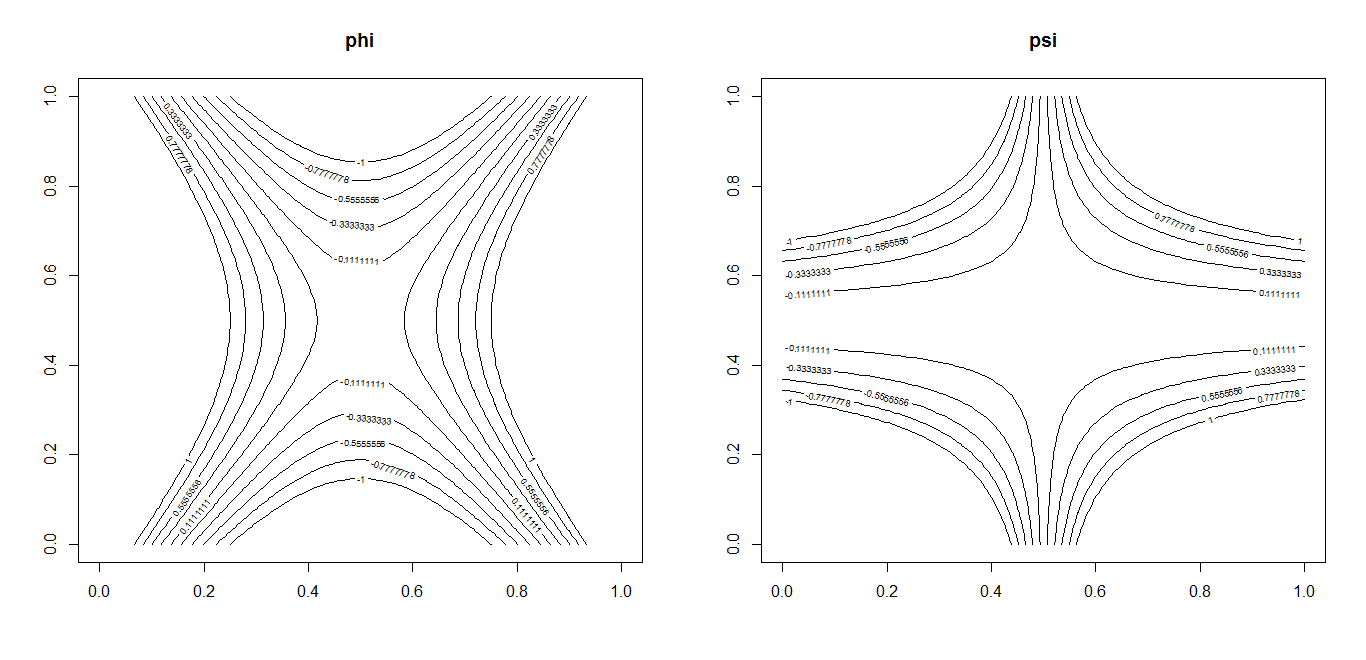
\includegraphics[scale=0.25]{c2f9}}
\caption{$\phi$ and $\psi$ for axisymmetric flow in cylindrical coordinates.}
\label{c2f9}
\end{figure}
The figures were generated using the code:
\begin{verbatim}
N <- 100
x <- seq(from = -2, to = 2, len = N)
sigma <- seq(from = -2, to = 2, len = N)

f1 <- function(x, sigma) { x^2 - sigma^2/2 }

f2 <- function(x, sigma) { x*sigma^2 }

lv <- seq(from = -1, to = 1, len = 10)
phi <- outer(x, sigma, FUN = 'f1')
psi <- outer(x, sigma, FUN = 'f2')

par(mfrow = c(1, 2))
contour(phi, levels = lv)
title('phi')
contour(psi, levels = lv)
title('psi')
\end{verbatim}
\end{itemize}

\section{Irrotational solenoidal flow in doubly-connected regions}
\begin{itemize}
\item We will show that although $\phi$ is multivalued in a doubly-connected region, $\vec{v}$ is not so. Let $\phi(\vec{x}, n)$ denote the value of $\phi$ at $\vec{x}$ after going 
aroung the cylinder $n$ times. Thus, $\phi(\vec{x}, n) = \phi(\vec{x}, 0) + n\kappa$. However, $\grad{\phi(\vec{x}, n)} = \grad{\phi(\vec{x}, 0)} + 0$, which means that the velocity 
$\vec{v}$ does not change by going around the cylinder.

\item Equation (2.6.6) of the books says
\[
\vec{u}_v(\vec{x}) = -\frac{\kappa}{4\pi}\grad{\Omega},
\]
where
\[
\Omega(\vec{x}) = \int\frac{\vec{s}\cdot\un}{s^3}dA(\vec{x}^\op)
\]
Since $\vec{v} = \grad{\phi}$, we observe that
\[
\phi(\vec{x}) = -\frac{\kappa}{4\pi}\Omega,
\]
where $\Omega$ is the solid angle subtended at $\vec{x}$ by the closed line vertex. If we go round the line vortex once, we cover a solid angle $\Omega + 4\pi$ so that $\phi$ gets an
additional value of $-\kappa$.

\item To prove equation (2.8.5), we use another, but equivalent, definition of a solid angle. The solid angle subtended by an area at a point is the area of a unit sphere centerd at the
point that is intersected by a cone joining the the point to the edges of the area. Refer to figure \ref{c2f3} for a picture of the cone. Let the line vortex be along the $z$ axis and let
it be turned into a loop by an infinite semicircle lying in the $yz$ plane. If the field point is on the negative $z$ azix, the cone collapes to a sheet and the region of intersection 
with the sphere reduces to zero, making the solid angle also zero. Let us use the negative $y$ axis as the \enquote*{zero} of the angle $\phi$. If $\vec{x}$ moves by $\pi/2$ to reside
on the positive $x$ axis, the generators of the cone are perpendicular to each other in the $xy$ plane. For one of them is along the $x$ axis and the other is perpendicular to it, running
parallel to the $y$ axis. If, instead, $\vec{x}$ moves only by an angle $\Theta$, the angle between the generators is also $\Theta$ as shown in figure \ref{c2f10}.
\begin{figure}[!ht]
\centering
\centerline{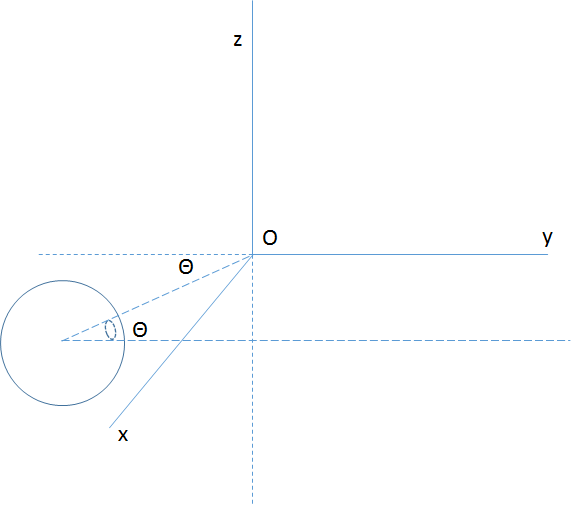
\includegraphics[scale=0.5]{c2f10}}
\caption{Solid angle subtended by an infinite line vortex.}
\label{c2f10}
\end{figure}
Note that the variables of integration in $\Omega$ are the coordinates with respect to a spherical polar coordinate system centerd at the unit sphere. Therefore, the solid angle 
subtended is
\[
\Omega = \int_0^{\pi}\int_{0}^{\Theta}\sin\theta d\theta d\varphi = \int_0^{\pi} \sin\theta d\theta \int_{0}^{\Theta} d\varphi = -2\Theta,
\]
so that,
\[
\phi(\vec{x}) = -\frac{\kappa}{4\pi}(-2\Theta) = \frac{\kappa}{2\pi}\Theta
\]
We assumed the field point in the $xy$ plane. There is no loss of generality in doing so because of the infinite extent of the line vortex.

\item In order to prove equation (2.8.9) of the book, note that $\vec{v}_1\cdot\vec{v}_2 = \grad{\phi}_1\cdot\grad{\phi}_2$. Now, 
\[
\dive{\phi_1\grad{\phi}_2} = \grad{\phi}_1\cdot\grad{\phi}_2 + \phi_1\nabla^2\phi_2
\]
Since $\phi_2$ is a harmonic function, $\nabla^2\phi_2 = 0$ so that $\grad{\phi}_1\cdot\grad{\phi}_2 = \dive{\phi_1\grad{\phi}_2}$ and hence,
\[
\int \vec{v}_1\cdot\vec{v}_2 dV = \int \dive{\phi_1\grad{\phi}_2} dV
\]
Using divergence theorem on the right hand side,
\[
\int \vec{v}_1\cdot\vec{v}_2 dV = \int \phi_1\grad{\phi}_2\cdot\un dA
\]
The bottom of page 113 showed that $\un\cdot\grad{\phi}_2 = 0$, making the right hand side of the above equation vanish.
\end{itemize}

\subsection{Exercise}
\begin{enumerate}
\item In equation (2.8.10), the left hand side is fixed by choice of the velocity of the fluid. It depends only on the volume and the external experimental conditions. The value of the 
integral $\kappa\int\phi_1\vec{v}_1\cdot\un dA$ is also fixed because $\phi_1$ is single valued and $\vec{v}_1\cdot\un$ is specified by the problem. Since two out of three terms are fixed 
by experiment, the third one too is fixed, that is, independent of choice of the barrier $S$.

In equation (2.8.8), although the LHS is fixed by experiment, since $\phi$ is not single valued, the term $\kappa\int\phi\vec{v}\cdot\un dA$ depends on the choice of the barrier. 
Therefore, the third and remaining term of the equation too depends on choice of the barrier $S$.
\end{enumerate}

\section{Three dimensional flow fields extending to infinity}\label{c2s9}
\begin{itemize}
\item Consider the expression for velocity field due to a given rate of expansion,
\[
\vec{u}_e = \frac{1}{4\pi}\int_0^\infty\int_0^{2\pi}\int_0^\pi \frac{\vec{s}}{s^3}\Delta(\vec{x}^\op){r^\op}^2\sin\theta^\op dr^\op d\theta^\op d\varphi^\op
\]
Divide the domain of integral into an inner spherical region of area $\alpha r$ and the one outside it. The right hand side than then be written as a sum of two integrals, $\vec{I}_1$ and
$\vec{I}_2$ of which
\[
\vec{I}_2 = \frac{1}{4\pi}\int_{\alpha r}^\infty\int_0^{2\pi}\int_0^\pi \frac{\vec{s}}{s^3}\Delta(\vec{x}^\op){r^\op}^2\sin\theta^\op dr^\op d\theta^\op d\varphi^\op
\]
Let $\Delta(\vec{x}^\op) = a{r^\op}^{-n}$. In the region of integration, $s \approx r$, where $r = |\vec{x}|$.  Therefore,
\[
\vec{I}_2 = \frac{1}{4\pi}\frac{\vec{r}}{r^3}\int_{\alpha r}^\infty\int_0^{2\pi}\int_0^\pi a{r^\op}^{-n} {r^\op}^2\sin\theta^\op dr^\op d\theta^\op d\varphi^\op
\]
or
\[
\vec{I}_2 = \frac{\uvec{r}}{r^2}\frac{a}{(\alpha r)^{-3 + n}} = \uvec{r} O(r^{-n + 1})
\]
Therefore, when the field point $\vec{x}$ is very far away from the source point $\vec{x}^\op$, we can approximate $\vec{u}_e(\vec{x})$ as
\[
\vec{u}_e = \frac{1}{4\pi}\int_0^{\alpha r}\int_0^{2\pi}\int_0^\pi \frac{\vec{x}}{x^3}\Delta(\vec{x}^\op){r^\op}^2\sin\theta^\op dr^\op d\theta^\op d\varphi^\op
\]
Since 
\[
\grad{\left(\frac{1}{r}\right)} = -\frac{\vec{x}}{x^3}
\]
where $r = |\vec{x}|$, we have
\[
\vec{u}_e = -\frac{1}{4\pi}\int_0^{\alpha r}\int_0^{2\pi}\int_0^\pi \grad{\left(\frac{1}{r}\right)} \Delta(\vec{x}^\op){r^\op}^2\sin\theta^\op dr^\op d\theta^\op d\varphi^\op
\]
or
\[
\vec{u}_e = 
-\frac{1}{4\pi}\grad{\left(\frac{1}{r}\right)}\left\{\int_0^{\alpha r}\int_0^{2\pi}\int_0^\pi \Delta(\vec{x}^\op){r^\op}^2\sin\theta^\op dr^\op d\theta^\op d\varphi^\op\right\}
\]
or, writing the integral more succinctly,
\[
\vec{u}_e = -\frac{1}{4\pi}\grad{\left(\frac{1}{r}\right)}\left\{\int \Delta(\vec{x}^\op)dV(\vec{x}^\op)\right\}
\]
If the integral $\smallint \Delta(\vec{x}^\op)dV(\vec{x}^\op)$ vanishes, we go to the next term in the Taylor expansion of $\vec{s}/s^3$ and write $\vec{u}_e(\vec{x})$ in terms of
the source dipole. Refer to point \ref{c2sa4} for the \enquote*{multipole} expansion of electrostatic field, which is analogous to $\vec{u}_e$.

\item Velocity field due to a given vorticity distribution is
\[
\vec{u}_v(\vec{x}) = -\frac{1}{4\pi}\int\frac{\vec{s}\vp\vec{\omega}(\vec{x}^\op)}{s^3} dV(\vec{x}^\op)
\]
Proceeding in similar was as we did for a given rate of expansion, for a localized vorticity distribution, we get
\begin{eqnarray*}
\vec{u}_v &=& \frac{1}{4\pi}\grad{\left(\frac{1}{r}\right)}\vp\left\{\int \vec{\omega}(\vec{x}^\op)dV(\vec{x}^\op)\right\} \\
 &=& -\frac{1}{4\pi}\left\{\int \vec{\omega}(\vec{x}^\op)dV(\vec{x}^\op)\right\} \vp \grad{\left(\frac{1}{r}\right)}
\end{eqnarray*}
Consider $\dive{(x_i\vec{\omega})} = \grad{x_i}\cdot\vec{\omega} + x_i\dive{\omega} = \uvec{i}\cdot\vec{\omega} = \omega_i$. Therefore,
\[
\int\vec{\omega}(\vec{x}^\op)dV(\vec{x}^\op) = \int\dive{(x_i^\op\vec{\omega}(\vec{x}^\op))}dV(\vec{x}^\op)
\]
Using divergence theorem on the right hand side,
\[
\int\vec{\omega}(\vec{x}^\op)dV(\vec{x}^\op) = \int x_i\vec{\omega}(\vec{x}^\op)\cdot\un dA
\]
If we choose $\alpha$ such that on the surface of the sphere of radius $\alpha r$, the vorticity is very small, then the right hand side of the above equation is zero.

\item We now prove the identity,
\[
\vec{A}\vp(\vec{B}\cdot\grad{\vec{f}}) = \curl{\left(\vec{A}(\vec{B}\cdot\vec{f})\right)},
\]
where $\vec{A}$ and $\vec{B}$ are constant vectors while $\vec{f}$ is an irrotational vector field. Starting from the right hand side,
\[
\curl{\left(\vec{A}(\vec{B}\cdot\vec{f})\right)} = (\curl{\vec{A}})(\vec{B}\cdot\vec{f}) + \vec{A}\vp\grad{(\vec{B}\cdot\vec{f})} 
\]
which follows immediately if we write $\phi(\vec{x}) = \vec{B}\cdot\vec{f}$. Since, $\vec{A}$ is a constant vector,
\[
\curl{\left(\vec{A}(\vec{B}\cdot\vec{f})\right)} = \vec{A}\vp\grad{(\vec{B}\cdot\vec{f})} 
\]
Now,
\[
\grad{(\vec{B}\cdot\vec{f})} = \vec{B}\cdot\grad{\vec{f}} + \vec{f}\cdot\grad{\vec{B}} + \vec{B}\vp\curl{\vec{f}} + \vec{f}\vp\curl{\vec{B}}
\]
Since $\vec{B}$ is a constant vector and $\vec{f}$ is an irrotational field,
\[
\grad{(\vec{B}\cdot\vec{f})} = \vec{B}\cdot\grad{\vec{f}} 
\]
Therefore,
\begin{equation}\label{c2s9e1}
\curl{\left(\vec{A}(\vec{B}\cdot\vec{f})\right)} = \vec{A}\vp\left(\vec{B}\cdot\grad{\vec{f}}\right)
\end{equation}

\item We go back to the velocity field due to a given vorticity distribution
\[
\vec{u}_v(\vec{x}) = -\frac{1}{4\pi}\int\frac{\vec{s}\vp\vec{\omega}(\vec{x}^\op)}{s^3} dV(\vec{x}^\op)
\]
and write it as
\[
\vec{u}_v(\vec{x}) = \frac{1}{4\pi}\int\grad{\left(\frac{1}{s}\right)}\vp\vec{\omega}(\vec{x}^\op) dV(\vec{x}^\op)
\]
We know that
\[
\frac{1}{s} = \frac{1}{r} + \vec{x}^\op\cdot\grad{\left(\frac{1}{s}\right)}
\]
When $r = |\vec{x}|$ is very large as compared to $r^\op = |\vec{x}^\op|$, we can approximate $s$ as $r$ so that
\[
\frac{1}{s} = \frac{1}{r} + \vec{x}^\op\cdot\grad{\left(\frac{1}{r}\right)}
\]
We saw previously that approximating $s^{-1}$ as $r^{-1}$ led to vanishing velocity. We therefore consider the second term to get
\[
\vec{u}_v(\vec{x}) = \frac{1}{4\pi}\int\grad{\left(\vec{x}^\op\cdot\grad{\left(\frac{1}{r}\right)}\right)}\vp\vec{\omega}(\vec{x}^\op) dV(\vec{x}^\op)
\]
Now since $\vec{x}^\op$ is a constant in a gradient operation,
\[
\grad{\left(\vec{x}^\op\cdot\grad{\left(\frac{1}{r}\right)}\right)} = \vec{x}^\op\cdot\grad{\left(\grad{\left(\frac{1}{r}\right)}\right)} + 
\vec{x}^\op\vp\curl{\left(\grad{\left(\frac{1}{r}\right)}\right)}
\]
Since curl of a gradient is always zero,
\[
\grad{\left(\vec{x}^\op\cdot\grad{\left(\frac{1}{r}\right)}\right)} = \vec{x}^\op\cdot\grad{\left(\grad{\left(\frac{1}{r}\right)}\right)} 
\]
so that
\[
\vec{u}_v(\vec{x}) = \frac{1}{4\pi}\int\vec{x}^\op\cdot\grad{\left(\grad{\left(\frac{1}{r}\right)}\right)}\vp\vec{\omega}(\vec{x}^\op) dV(\vec{x}^\op)
\]
or
\[
\vec{u}_v(\vec{x}) = -\frac{1}{4\pi}\int\vec{\omega}(\vec{x}^\op)\vp\left\{\vec{x}^\op\cdot\grad{\left(\grad{\left(\frac{1}{r}\right)}\right)}\right\}dV(\vec{x}^\op)
\]
From \eqref{c2s9e1},
\[
\vec{u}_v(\vec{x}) = -\frac{1}{4\pi}\int\curl{\left\{\vec{\omega}(\vec{x}^\op)\left(\vec{x}^\op\cdot\grad{\left(\frac{1}{r}\right)}\right)\right\}}dV(\vec{x}^\op)
\] 
Since curl is with respect to unprimed coordinates.
\begin{equation}\label{c2s9e2}
\vec{u}_v(\vec{x}) = -\frac{1}{4\pi}\curl\int \vec{\omega}(\vec{x}^\op) \left(\vec{x}^\op\cdot\grad{\left(\frac{1}{r}\right)}\right) dV(\vec{x}^\op)
\end{equation}

\item We will now prove that 
\[
\int(x_i\omega_j + x_j\omega_i)dV = 0
\]
and if $\omega$ decays faster than $r^{-4}$, the right hand side is zero. Consider
\[
\dive{(x_ix_j\vec{\omega})} = \grad{(x_ix_j)}\cdot\vec{\omega} + x_ix_j\dive{\vec{\omega}} = \grad{(x_ix_j)}\cdot\vec{\omega}
\]
Now, $\grad{(x_ix_j)} = x_i\grad{x_j} + x_j\grad{x_i} = x_i\delta_{kj}\uvec{k} + x_j\delta_{ik}\uvec{k} = x_i\uvec{j} + x_j\uvec{i}$ so that
\[
\grad{(x_ix_j)}\cdot\vec{\omega} = (x_i\uvec{j} + x_j\uvec{i})\cdot\vec{\omega} = x_i\omega_j + x_j\omega_i
\]
and hence
\[
\int\dive{(x_ix_j\vec{\omega})}dV = \int(x_i\omega_j + x_j\omega_i)dV
\]
The left hand side can be written as
\[
\int (x_i x_j \vec{\omega})\cdot\un dA
\]
If $\omega$ decays faster than $r^{-4}$ then the volume over which we integrated can be made large enough so that $\omega$ is almost zero on its surface making
\begin{equation}\label{c2s9e3}
\int(x_i\omega_j + x_j\omega_i)dV = 0
\end{equation}
Writing in Gibbs vector form,
\begin{equation}\label{c2s9e4}
\int(\vec{x}\vec{\omega} + \vec{\omega}\vec{x})dV = 0
\end{equation}

\item An immediate consequence of \eqref{c2s9e4} is that if $\vec{f}$ is a vector field 
\begin{equation}\label{c2s9e5}
\int(\vec{x}\vec{\omega}\cdot\vec{f} + \vec{\omega}\vec{x}\cdot\vec{f})dV = 0
\end{equation}
so that
\[
-\int \vec{\omega}\vec{x}\cdot\vec{f}dV = -\int \vec{\omega}\vec{x}\cdot\vec{f}dV + \frac{1}{2}\int(\vec{x}\vec{\omega}\cdot\vec{f} + \vec{\omega}\vec{x}\cdot\vec{f})dV
\]
or
\[
-\int \vec{\omega}\vec{x}\cdot\vec{f}dV = \frac{1}{2}\int(\vec{x}\vec{\omega}\cdot\vec{f} - \vec{\omega}\vec{x}\cdot\vec{f})dV
\]
If $\vec{f} = \grad{(1/r)}$,
\[
-\int \vec{\omega}\vec{x}\cdot\grad{\left(\frac{1}{r}\right)}dV = \frac{1}{2}\int(\vec{x}\vec{\omega}\cdot\grad{\left(\frac{1}{r}\right)} - 
\vec{\omega}\vec{x}\cdot\grad{\left(\frac{1}{r}\right)}dV
\]
Since
\[
\grad{\left(\frac{1}{r}\right)}\vp\left(\vec{\omega}(\vec{x}^\op)\vp\vec{x}^\op\right) = \vec{\omega}(\vec{x}^\op)\grad{\left(\frac{1}{r}\right)}\cdot\vec{x}^\op - 
\vec{x}^\op\grad{\left(\frac{1}{r}\right)}\cdot\vec{\omega}(\vec{x}^\op)
\]
we have
\[
\vec{x}^\op\grad{\left(\frac{1}{r}\right)}\cdot\vec{\omega}(\vec{x}^\op) - \vec{\omega}(\vec{x}^\op)\grad{\left(\frac{1}{r}\right)}\cdot\vec{x}^\op = 
-\grad{\left(\frac{1}{r}\right)}\vp\left(\vec{\omega}(\vec{x}^\op)\vp\vec{x}^\op\right)
\]
so that
\[
-\int\vec{\omega}(\vec{x}^\op)\vec{x}^\op\cdot\grad{\left(\frac{1}{r}\right)}dV = -\frac{1}{2}\int\grad{\left(\frac{1}{r}\right)}\vp\left(\vec{\omega}(\vec{x}^\op)\vp\vec{x}^\op\right)dV
\]
or
\[
-\int\vec{\omega}(\vec{x}^\op)\vec{x}^\op\cdot\grad{\left(\frac{1}{r}\right)}dV = \frac{1}{2}\int\grad{\left(\frac{1}{r}\right)}\vp\left(\vec{x}^\op\vp\vec{\omega}(\vec{x}^\op)\right)dV
\]
From \eqref{c2s9e2},
\[
\vec{u}_v(\vec{x}) = \frac{1}{8\pi}\curl\int \grad{\left(\frac{1}{r}\right)}\vp\left(\vec{x}^\op\vp\vec{\omega}(\vec{x}^\op)\right) dV(\vec{x}^\op)
\]
or
\begin{equation}\label{c2s9e6}
\vec{u}_v(\vec{x}) = \frac{1}{8\pi}\curl\left\{\grad{\left(\frac{1}{r}\right)}\vp\int\left(\vec{x}^\op\vp\vec{\omega}(\vec{x}^\op)\right) dV(\vec{x}^\op)\right\}
\end{equation}
If $\vec{A}$ is a constant vector and $\vec{f}$ is a function of $\vec{x}$ then $\grad{(\vec{A}\cdot\vec{f})} = \vec{A}\cdot\grad{\vec{f}} + \vec{A}\vp\curl{\vec{f}}$ and
$\curl{(\vec{f}\vp\vec{A})} = -\vec{A}\dive{\vec{f}} + \vec{A}\cdot\grad{\vec{f}}$. Using the first equation in the second, we get
\[
\curl{(\vec{f}\vp\vec{A})} = -\vec{A}\dive{\vec{f}} + \grad{(\vec{A}\cdot\vec{f})} - \vec{A}\vp\curl{\vec{f}}
\]
If $\vec{f} = \grad{(1/r)}$, then its curl and divergence are zero so that
\[
\curl{\left(\grad{\left(\frac{1}{r}\right)}\vp\vec{A}\right)} = \grad{\left(\grad{\left(\frac{1}{r}\right)}\cdot\vec{A}\right)}
\]
Using this in \eqref{c2s9e6}, we get
\begin{equation}\label{c2s9e7}
\vec{u}_v(\vec{x}) = \frac{1}{8\pi}\grad{\left(\grad{\left(\frac{1}{r}\right)}\cdot\int\left(\vec{x}^\op\vp\vec{\omega}(\vec{x}^\op)\right) dV(\vec{x}^\op)\right)}
\end{equation}
The book uses an approximation sign instead of equality because this relation is true only very far away from the source.

\item In the section on the behaviour of $\phi$ at large distances, the analysis begins with Green's theorem whose requirements are that the functions $F$ and $G$ be single-valued, finite
and continuous throughout the volume of integration. The same restrictions are placed on derivatives of $F$ and $G$. These requirements force us to exclude the point $P$ from the region
of integration by enclosing it in a sphere of radius $\epsilon$.

\item In order to get (2.9.9) we evaluate the limit
\[
L = -\lim_{\epsilon \rightarrow 0}\int \left(\phi(\vec{x}^\op)\pdt{s^{-1}}{s} - \frac{1}{s}\pdt{\phi(\vec{x}^\op)}{s}\right)\Big|_{s = \epsilon} \epsilon^2 d\Omega(\vec{x}^\op)
\]
The integrand is simplified as
\[
-\frac{\phi(\vec{x}^\op)}{s^2} - \frac{1}{s}\pdt{\phi(\vec{x}^\op)}{s} = -\frac{1}{s^2}\left(\phi(\vec{x}^\op) + s\pdt{\phi(\vec{x}^\op)}{s}\right)
\]
Noting that the position vector of $P$ is $\vec{x}$ we replace the primed variable with the unprimed one. Evaluated at $s = \epsilon$ it is
\[
-\frac{1}{\epsilon^2}\left(\phi(\vec{x}) + \epsilon\pdt{\phi(\vec{x})}{s}\right) = -\frac{\phi(\vec{x} + \vec{\epsilon})}{\epsilon^2},
\]
where $\vec{\epsilon}$ is the radius vector of the sphere around $P$. We further get,
\[
L = +\lim_{\epsilon \rightarrow 0}\int\frac{\phi(\vec{x} + \vec{\epsilon})}{\epsilon^2}\epsilon^2 d\Omega(\vec{x}) = 4\pi\phi(\vec{x})
\]

\item After accounting for the above term, equation (2.9.8) of the book becomes
\[
\left.
\begin{array}{l}
\int(F\grad{G} - G\grad{F})\cdot\un_2dA_2 - \\
\int(F\grad{G} - G\grad{F})\cdot\un_1dA_1 + \\
+ 4\pi\phi(\vec{x}) 
\end{array}
\right\} = \int(F\nabla^2G - G\nabla^2F)dV
\]
If $F(\vec{x}^\op) = \phi(\vec{x}^\op)$ and $G(\vec{x}^\op) = s^{-1}$ then the right hand side of the above equation is zero and
\[
4\pi\phi(\vec{x}) = \int(F\grad^\op{G} - G\grad^\op{F})\cdot\un_1dA_1 - \int(F\grad^\op{G} - G\grad^\op{F})\cdot\un_2dA_2,
\]
where $\grad^\op$ denotes the gradient with respect to primed coordinates. Let $T_2$ denote the second term.
\begin{eqnarray*}
T_2 &=& \int(F\grad^\op{G} - G\grad^\op{F})\cdot\un_2dA_2 \\
 &=& \int\left(\phi(\vec{x}^\op)\grad^\op{\left(\frac{1}{s}\right)} - \left(\frac{1}{s}\right)\grad^\op{\phi(\vec{x}^\op)}\right)\cdot\un_2 dA_2 \\
\end{eqnarray*}
Since $A_2$ is the surface of a sphere of radius $R$,
\[
T_2 = -\frac{1}{R^2}\int \phi(\vec{x}^\op) dA_2 - \frac{1}{R}\int\grad^\op{\phi(\vec{x}^\op)}\cdot\un_2 dA_2
\]
Since $\dive{\vec{v}} = 0$ everywhere in $V$,
\[
\int\dive{\vec{v}}dV = 0
\]
or
\[
\int\vec{v}\cdot\un_2 dA_2 - \int\vec{v}\cdot\un_1 dA_1 = 0
\]
Let
\[
\int\grad^\op{\phi}(\vec{x}^\op)\cdot\un_2 dA_2 = \int\grad^\op{\phi}(\vec{x}^\op)\cdot\un_1 dA_1 = m,
\]
say so that
\[
T_2 = -\frac{1}{R^2}\int \phi(\vec{x}^\op) dA_2 - \frac{m}{R} = 4\pi\langle\phi(\vec{x}, R)\rangle - \frac{m}{R},
\]
where $\langle\cdot\rangle$ denotes the average. Thus,
\[
4\pi\phi(\vec{x}) = \int(F\grad^\op{G} - G\grad^\op{F})\cdot\un_1dA_1 + 4\pi\langle\phi(\vec{x}, R)\rangle - \frac{m}{R}
\]
or
\[
\phi(\vec{x}) = \langle\phi(\vec{x}, R)\rangle - \frac{m}{4\pi R} + \frac{1}{4\pi}\int\left(\phi(\vec{x}^\op)\grad^\op{\left(\frac{1}{s}\right)} - 
\left(\frac{1}{s}\right)\grad^\op{\phi(\vec{x}^\op)}\right)\cdot\un_1dA_1
\]
Note that the gradients in the integrand are all with respect to primed coordinates. If we want them to be in terms of un-primed coordinates, we get an overall negative sign to the 
integral.
\begin{equation}\label{c2s9e8}
\phi(\vec{x}) = \langle\phi(\vec{x}, R)\rangle - \frac{m}{4\pi R} - \frac{1}{4\pi}\int\left(\phi(\vec{x}^\op)\grad{\left(\frac{1}{s}\right)} - 
\left(\frac{1}{s}\right)\grad{\phi(\vec{x}^\op)}\right)\cdot\un_1dA_1
\end{equation}

\item We can write the equation for flux of $\phi$ as
\[
m = \int\grad^\op{\phi}(\vec{x}^\op)\cdot\un_2 dA_2 = R^2\int \left(\pdt{\phi(\vec{x}^\op)}{s}\right)_{s=R} d\Omega(\vec{x}^\op)
\]
Pulling out the differential operator (reverse of integration under the differential sign),
\[
m = R^2\frac{\partial}{\partial R}\int \left(\phi(\vec{x}^\op)\right)_{s=R} d\Omega(\vec{x}^\op)
\]
or,
\[
\frac{m dR}{R^2} = \partial\int \left(\phi(\vec{x}^\op)\right)_{s=R} d\Omega(\vec{x}^\op)
\]
or
\[
4\pi C - \frac{m}{R} = \int \left(\phi(\vec{x}^\op)\right)_{s=R} d\Omega(\vec{x}^\op),
\]
where $C$ is a constant of integration. Using the definition of $\langle\phi(\vec{x}, R)\rangle$, we see that
\[
\langle\phi(\vec{x}, R)\rangle = C - \frac{m}{4\pi R}
\]

\item Since $R$ is a fixed constant, $\grad{\langle\phi(\vec{x}, R)\rangle} = \grad{C}$ so that
\[
\grad{C} = \grad{\left(\frac{1}{4\pi R^2}\int\phi(\vec{x}^\op)\cdot\un dA_2\right)} = \frac{1}{4\pi R^2}\int\grad{\vec{x}^\op}\cdot\un dA_2
\]
or
\[
\grad{C} = -\frac{1}{4\pi R^2}\int\grad^\op{\vec{x}^\op}\cdot\un dA_2 = -\frac{1}{4\pi R^2}\int\vec{v}\cdot\un dA_2
\]
Since $\vec{v}$ is zero on the outer boundary, we see that $\vec{C} = 0$ or that $C$ is independent of $R$.

\item Since
\[
C = \langle\phi(\vec{x}, R)\rangle + \frac{m}{4\pi R}
\]
we can write \eqref{c2s9e8} as
\[
\phi(\vec{x}) = C - \frac{1}{4\pi}\int\left(\phi(\vec{x}^\op)\grad{\left(\frac{1}{s}\right)} - \left(\frac{1}{s}\right)\grad{\phi(\vec{x}^\op)}\right)\cdot\un_1dA_1
\]
This does not appear to be a very encouraging equation because $\phi$ appears on the right hand side as well. It appears as \enquote*{prescribed value} of $\phi$ on the inner boundary.
The book mentions that it can be converted \emph{in principle} into the prescribed value of $\grad{\phi}\cdot\un$ on the surface, although it does not tell how so.

\item We observed that 
\[
\int\vec{v}\cdot\vec{v}dV = \int\dive{(\phi\vec{v})}dV
\]
Since $\vec{v}$ is a solenoidal field, $\vec{v}\cdot\vec{v}$ is also equal to $\dive{\left((\phi - C)\vec{v}\right)}$.
Applying this relation in the present context,
\[
\int\vec{v}\cdot\vec{v}dV = \lim_{R \rightarrow \infty}\int\left((\phi - C)\vec{v}\right)\cdot\un_2 dA_2 - \int\left((\phi - C)\vec{v}\right)\cdot\un_1 dA_1
\]
The limit is applicable only to the first term because the inner boundary is fixed while the outer, spherical one is assumed to be at an infinite distance. Since $\phi(\vec{x}) 
\rightarrow C$ in the limit $R \rightarrow \infty$, the first term goes to zero and
\[
\int\vec{v}\cdot\vec{v}dV = - \int\left((\phi - C)\vec{v}\right)\cdot\un_1 dA_1
\]
or
\[
\int\vec{v}\cdot\vec{v}dV = -\int\phi\vec{v}\cdot\un dA_1 + C\int\vec{v}\cdot\un_1 dA_1 = -\int\phi\vec{v}\cdot\un dA_1 + Cm,
\]
where $m$ is the flux of $\phi$.

\item We previously observed that (see bottom of page 87 of the book) that $\vec{v}$ is determined from the prescribed boundary conditions. We will find $\vec{v}$ under the condition
$\vec{v}\cdot\un = \vec{U}\cdot\un$, where $\vec{U}$ is the velocity of a rigid body in a translational motion in the fluid, which is at rest at infinity. Thus, the mathematical 
statement of the problem is - solve $\nabla^2\phi = 0$ subject to the boundary conditions
\begin{enumerate}
\item $\phi(\vec{x}) \rightarrow$ a constant as $r = |\vec{x}| \rightarrow \infty$. We can choose the constant to be zero.
\item $\un\cdot\grad{\phi} = \un\cdot\vec{U}$
\end{enumerate}
We try a solution of the form $\phi(\vec{x}) = \vec{U}\cdot\vec{\Phi}(\vec{x})$, where $\vec{\Phi}$ is independent of $\vec{U}$. Since $\vec{\Phi}$ is determined by the boundary
condition on the surface of the rigid body, its value depends not on $\vec{x}$ but on its position vector with respect to an arbitrarily chosen material point, say $\vec{x}_0$, of the 
body. Thus,
\[
\phi(\vec{x}) = \vec{U}\cdot\vec{\Phi}(\vec{x} - \vec{x}_0)
\]
For a spherically symmetric body with its center instantaneously at the origin, $\vec{x}_0 = 0$. Further,
\[
\nabla^2\phi = \nabla^2(U_i\Phi_i) = U_i\nabla^2\Phi_i
\]
Since $U_i$ is, in general, not zero, $\nabla^2\phi = 0$ implies $\nabla^2\Phi_i = 0$ or $\nabla^2\vec{\Phi} = 0$. A solution of Laplace's equation which is also a component of a vector
is
\[
\frac{\partial}{\partial x_i}\left(\frac{1}{r}\right)
\]
Therefore, 
\[
\vec{\Phi} = \alpha\grad{\left(\frac{1}{r}\right)},
\]
where $\alpha$ is an arbitrary constant. Therefore,
\[
\phi(\vec{x}) = \alpha\vec{U}\cdot\grad{\left(\frac{1}{r}\right)} = -\alpha\frac{\vec{U}\cdot\vec{x}}{r^3}
\]
and hence,
\begin{eqnarray*}
\vec{v} &=& \grad{\phi} \\
 &=& -\alpha\grad{\left[\vec{U}\cdot\grad{\left(\frac{1}{r}\right)}\right]} \\
 &=& -\alpha(\vec{U}\cdot\nabla)\grad{\left(\frac{1}{r}\right)} - \alpha\vec{U}\vp\left\{\curl{\grad{\left(\frac{1}{r}\right)}}\right\}
\end{eqnarray*}
Since curl of a gradient is always zero,
\[
\vec{v} = -\alpha(\vec{U}\cdot\nabla)\grad{\left(\frac{1}{r}\right)}
\]
\end{itemize}

\section{Two dimensional flow fields extending to infinity}\label{c2s10}
\begin{itemize}
\item A two dimensional motion is the one whose velocity field is of the form $\vec{u}(x, y) = (u, v, 0)$ or equivalent. A two dimensional flow field extending to infinity is the one
which extends to infinity in $x$ and $y$ (or any other pair) of directions. It is either bounded in the $z$ (or the remaining) direction or it extends to infinity without motion 
diminishing as one travels along the $z$ direction. In such a flow field, the assumption made in the previous section that the velocity on the outer sphere is zero does not hold good.
That is why it needs a separate treatment.

\item The construct of a large sphere, centered at the field point and including all internal boundaries is used only to examine the behaviour of $\phi$. Therefore, all formulae in 
section 2.9 of the book, up to equation (2.9.7), are applicable to two dimensional flow fields.

\item It is possible to use equation (2.9.8) of the book for the plane by replacing $dV$ by $dA$ and $dA$ by $dl$ because the divergence theorem can be \href{http://mathworld.wolfram.com/
DivergenceTheorem.html}{applied to plane} as well. Refer to sub section \ref{c2sa9} for a proof.

\item We saw in section \ref{c2sa6} that $\ln|\vec{x} - \vec{x}^\op|$ is a solution of Laplace's equation in two dimensions. That is why we choose $F(\vec{x}^\op) = \phi(\vec{x}^\op)$
and $G(\vec{x}^\op) = \ln s$ in equation(2.9.8). Doing so, we get
\begin{eqnarray*}
\int\grad^\op(\phi(\vec{x}^\op)\ln s)\cdot d\vec{l}^\op_2 - \int\grad^\op(\phi(\vec{x}^\op)\ln s)\cdot d\vec{l}^\op_1 &=& \\ 
\int(\phi(\vec{x}^\op){\nabla^\op}^2\ln s - \ln s {\nabla^\op}^2\phi(\vec{x}^\op))dA^\op, & &
\end{eqnarray*}
where the subscript $1$ to $\nabla$ indicates differentiation with respect to the primed coordinates. The function $\ln s$ blows up at the field point $\vec{x}$. Therefore, we exclude 
it by enclosing it in a small circle of radius $\epsilon$ centerd at $\vec{x}$. The exclusion appears on the left hand side in the form of an additional term
\[
L = -\lim_{\epsilon \rightarrow 0}\int\left(\phi(\vec{x}^\op)\pdt{(\ln s)}{s} - \ln s\pdt{\phi(\vec{x}^\op)}{s}\right)\Big|_{s=\epsilon}\epsilon d\theta
\]
Interchanging the order of integration and limit the integrand is,
\[
\lim_{\epsilon \rightarrow 0}\left(\frac{\phi(\vec{x}^\op)}{\epsilon} - \ln\epsilon\pdt{\phi(\vec{x}^\op)}{s}\Big|_{s=\epsilon} \right) \epsilon = \phi(\vec{x}^\op),
\]
because 
\[
\lim_{\epsilon \rightarrow 0}\epsilon\ln\epsilon = 0,
\]
by l'H\^{o}pital's rule. Therefore, $L = -2\pi\phi(\vec{x}^\op)$. Since $\phi$ and $\ln s$ are harmonic functions, the right hand side of the 2d analog of (2.9.8) is
\[
\int\grad^\op(\phi(\vec{x}^\op)\ln s)\cdot d\vec{l}^\op_2 - \int\grad^\op(\phi(\vec{x}^\op)\ln s)\cdot d\vec{l}^\op_1 - 2\pi\phi(\vec{x}^\op) = 0
\]
or
\[
\phi(\vec{x}) = \frac{1}{2\pi}\int\grad^\op(\phi(\vec{x}^\op)\ln s)\cdot d\vec{l}^\op_2 - \frac{1}{2\pi}\grad^\op\int(\phi(\vec{x}^\op)\ln s)\cdot d\vec{l}^\op_1
\]
Since the first integral on the right hand side is taken over a circle of radius $R$ centerd at $\vec{x}$,
\begin{equation}\label{c2s10e1}
\phi(\vec{x}) = \frac{1}{2\pi R}\int\phi(\vec{x}^\op)dl^\op_2 + \frac{\ln R}{2\pi}\int\grad^\op{\phi(\vec{x}^\op)}\cdot d\vec{l}^\op_2 - 
\frac{1}{2\pi}\int\grad^\op(\phi(\vec{x}^\op)\ln s)\cdot d\vec{l}^\op_1
\end{equation}
Now,
\[
\frac{1}{2\pi R}\int\phi(\vec{x}^\op)dl^\op_2  = \langle\phi\rangle,
\]
the mean value of $\phi$ over the outer boundary while
\[
-\int\grad^\op{\phi(\vec{x}^\op)}\cdot d\vec{l}^\op_2 = \int\grad{\phi(\vec{x}^\op)}\cdot d\vec{l}^\op_2 = m,
\]
is the flux through it, so that \eqref{c2s10e1} becomes,
\begin{equation}\label{c2s10e2}
\phi(\vec{x}) = \langle\phi\rangle - \frac{m}{2\pi}\ln R - \frac{1}{2\pi}\int\grad^\op(\phi(\vec{x}^\op)\ln s)\cdot d\vec{l}^\op_1
\end{equation}

\item The analog of the flux relation (2.9.10) is
\[
m = \int\grad^\op\phi(\vec{x}^\op)\cdot d\vec{l}^\op_2
\]
Over a circle of radius $R$ centerd at $\vec{x}$,
\[
m = R\int\pdt{\phi}{s}\Big|_{s=R} d\theta(\vec{x}^\op) = R\frac{\partial}{\partial R}\int\phi(\vec{x}^\op)\Big|_{s=R}d\theta(\vec{x}^\op)
\]
or
\[
m\ln R = \int\phi(\vec{x}^\op)\Big|_{s=R}d\theta(\vec{x}^\op) - 2\pi C,
\]
where $C$ is a constant of integration. Thus,
\[
\frac{m}{2\pi}\ln R = \langle\phi\rangle - C
\]
so that equation \eqref{c2s10e2} becomes
\[
\phi(\vec{x}) = C - \frac{1}{2\pi}\int\grad^\op(\phi(\vec{x}^\op)\ln s)\cdot d\vec{l}^\op_1
\]
In terms of derivative with respect to unprimed coordinates,
\[
\phi(\vec{x}) = C + \frac{1}{2\pi}\int\grad{(\phi(\vec{x}^\op)\ln s)}\cdot d\vec{l}^\op_1
\]
or
\begin{equation}\label{c2s10e3}
\phi(\vec{x}) = C + \frac{1}{2\pi}\int\left(\phi(\vec{x}^\op)\grad\ln s + \ln s\grad\phi(\vec{x}^\op)\right)\cdot d\vec{l}^\op_1
\end{equation}
or
\[
\phi(\vec{x}) - C = \frac{1}{2\pi}\int\left(\frac{\phi(\vec{x}^\op)}{s} + \ln s\grad\phi(\vec{x}^\op)\right)\cdot d\vec{l}^\op_1
\]
or
\[
\phi(\vec{x}) - C - \frac{m}{2\pi}\ln r = \frac{1}{2\pi}\int\left(\frac{\vec{s}}{s}\phi(\vec{x}^\op) + \ln s\grad\phi(\vec{x}^\op)\right)\cdot d\vec{l}^\op_1 - \frac{m}{2\pi}\ln r
\]
Using the fact that
\[
m = \int\grad^\op\phi(\vec{x}^\op)\cdot d\vec{l}^\op_2
\]
on the right hand side we get
\[
\phi(\vec{x}) - C - \frac{m}{2\pi}\ln r = \frac{1}{2\pi}\int\left(\frac{\vec{s}}{s}\phi(\vec{x}^\op) + \ln\frac{s}{r}\grad\phi(\vec{x}^\op)\right)\cdot d\vec{l}^\op_1
\]
Unlike the three dimensional case, as $r \rightarrow \infty$, it is not $\phi$ but 
\[
\phi(\vec{x}) - \frac{m}{2\pi}\ln r
\]
that tends to $C$. We need the term $m\ln r/(2\pi)$ because it creates the term $\ln(s/r)$, whose argument to $1$ as $r \rightarrow \infty$.

\item We can reconcile the behaviour in two and three dimensions if we state that it is the difference between the velocity potential and the source term that tends to a constant as 
$r \rightarrow \infty$. In three dimensions, the source term being of $O(r^{-1})$ itself vanishes at infinity. On the other hand, in two dimensions, the source term rises logarithmically
at infinity.

\item We first observe that
\begin{eqnarray*}
\left[\vec{v} - \grad\left(\frac{m}{2\pi}\ln r\right)\right]\cdot\left[\vec{v} - \grad\left(\frac{m}{2\pi}\ln r\right)\right] &=& \\ 
\dive\left\{\left[\phi - C - \left(\frac{m}{2\pi}\ln r\right)\right]\left[\vec{v} - \grad\left(\frac{m}{2\pi}\ln r\right)\right]\right\} & & 
\end{eqnarray*}
This is because $\vec{v}$ is a solenoidal field and $\ln r$ is a harmonic function. Therefore,
\begin{eqnarray*}
\int\left[\vec{v} - \grad\left(\frac{m}{2\pi}\ln r\right)\right]\cdot\left[\vec{v} - \grad\left(\frac{m}{2\pi}\ln r\right)\right]dA &=& \\ 
\int\dive\left\{\left[\phi - C - \left(\frac{m}{2\pi}\ln r\right)\right]\left[\vec{v} - \grad\left(\frac{m}{2\pi}\ln r\right)\right]\right\}dA & & 
\end{eqnarray*}
Using divergence theorem in the plane (refer to \ref{c2sa9}) on the right hand side
\begin{eqnarray*}
\int\left[\vec{v} - \grad\left(\frac{m}{2\pi}\ln r\right)\right]\cdot\left[\vec{v} - \grad\left(\frac{m}{2\pi}\ln r\right)\right]dA &=& \\ 
\int\left\{\left[\phi - C - \left(\frac{m}{2\pi}\ln r\right)\right]\left[\vec{v} - \grad\left(\frac{m}{2\pi}\ln r\right)\right]\right\}\cdot\un_2 dl - & & \\
\int\left\{\left[\phi - C - \left(\frac{m}{2\pi}\ln r\right)\right]\left[\vec{v} - \grad\left(\frac{m}{2\pi}\ln r\right)\right]\right\}\cdot\un_1 dl & & 
\end{eqnarray*}
Choose the outer boundary as large as possible by making the radius of the outer circle tend to infinity. In this limit the integrand tends to zero and hence,
\begin{eqnarray*}
\int\left[\vec{v} - \grad\left(\frac{m}{2\pi}\ln r\right)\right]\cdot\left[\vec{v} - \grad\left(\frac{m}{2\pi}\ln r\right)\right]dA &=& \\ 
-\int\left\{\left[\phi - C - \left(\frac{m}{2\pi}\ln r\right)\right]\left[\vec{v} - \grad\left(\frac{m}{2\pi}\ln r\right)\right]\right\}\cdot\un_1 dl & & 
\end{eqnarray*}
If
\begin{eqnarray*}
\Phi &=& \phi - \left(\frac{m}{2\pi}\ln r\right) \\
\vec{V} &=& \vec{v} - \grad\left(\frac{m}{2\pi}\ln r\right)
\end{eqnarray*}
then the previous equation becomes,
\[
\int\vec{V}\cdot\vec{V}dA = -\int(\Phi - C)\vec{V}\cdot\un_1 dl
\]
Now let, if possible, $\Phi$ and $\Phi^\ast$ be two solutions of Laplace's equation in two dimensions with identical boundary conditions. Then $\Phi - \Phi^\ast$ too will be a solution 
and
\[
\int(\vec{V} - \vec{V}^\ast)\cdot(\vec{V} - \vec{V}^\ast)dA = -\int\left((\Phi - \Phi^\ast) - (C - C^\ast)\right)(\vec{V} - \vec{V}^\ast)\cdot\un_1 dl
\]
By virtue of boundary conditions, $\grad{\phi}\cdot\un = \vec{v}\cdot\un$ is identical on the boundary for both solutions. Since the factor $m\ln r/(2\pi)$ is same for both solutions,
\[
\vec{V}\cdot\un = \vec{V}^\ast\cdot\un
\]
on the boundary. Therefore the right hand side is zero making
\[
\int(\vec{V} - \vec{V}^\ast)\cdot(\vec{V} - \vec{V}^\ast)dA = 0,
\]
which is possible only if $\vec{V} = \vec{V}^\ast$. Thus, in two dimensions the unique solution of Laplace equation is
\[
\phi - \left(\frac{m}{2\pi}\ln r\right) 
\]
\end{itemize}

\section{Exercises}\label{c2s11}
\begin{enumerate}
\item Consider a material line element joining points $P$ and $Q$. Let $r$ be the length of the material line element. If $\vec{x}_0$ is the position vector of $P$ then that of $Q$ is 
$\vec{x}_0 + r\uvec{r}$, where $\uvec{r}$ is a unit vector parallel to the line element, at a certain instance of time. Let, after a time $\delta t$, $P$ get to $\vec{x}_0 + \vec{X}$ so
 that $Q$ goes to $(\vec{x}_0 + r\uvec{r}) + r\uvec{r}\cdot\grad\vec{X}$, where we have ignored terms of higher order in $r\uvec{r}$. If the line element was along $r\uvec{r}$ 
initially, it is now along $q\uvec{q} = r(\uvec{r} + \uvec{r}\cdot\grad\vec{X})$. Thus,
\[
q^2 = r^2(1 + 2\uvec{r}\cdot\grad\vec{X}\cdot\uvec{r}),
\]
where we have ignored terms higher than second order in $\uvec{r}$. Thus,
\[
\frac{q^2}{r^2} = 1 + 2\uvec{r}\cdot\grad\vec{X}\cdot\uvec{r}
\]
or
\[
\frac{q}{r} = \left(1 + 2\uvec{r}\cdot\grad\vec{X}\cdot\uvec{r}\right)^{1/2} = 1 + \uvec{r}\cdot\grad\vec{X}\cdot\uvec{r}
\]
or
\[
\frac{q}{r} - 1 = \frac{q - r}{r} = \uvec{r}\cdot\grad\vec{X}\cdot\uvec{r}
\]
The quantity $(q - r)/r$ is the strain of the element, $\lambda$. Therefore, the rate of change of strain is,
\[
\td{\lambda}{t} = \uvec{r}\cdot\grad\vec{U}\cdot\uvec{r},
\]
where $\vec{U}$ is the velocity of $Q$ relative to $P$. We can as well write it as
\[
\td{\lambda}{t} = \frac{\vec{r}\cdot\grad\vec{U}\cdot\vec{r}}{r^2}
\]
The quantity $\vec{r}\cdot\grad\vec{U}\cdot\vec{r}$ is the rate-of-strain ellipsoid centerd at $P$. The point $Q$ lies on it. If one imagines a sphere centered at $P$ and of radius $r$ 
then $Q$ lies on it in the unstrained state. As time goes by, the point $Q$ finds itself on the ellipsoid described by $\vec{r}\cdot\grad\vec{U}\cdot\vec{r}$.

\item Given that
\[
\vec{B}_v(\vec{x}) = \frac{1}{4\pi}\int\frac{\vec{\omega}(\vec{x}^{\op})}{s}dV(\vec{x}^{\op}) - \frac{1}{4\pi}\int\frac{\un\vp\vec{u}(\vec{x}^{\op})}{s}dA(\vec{x}^{\op})
\]
Therefore,
\[
\curl\vec{B}_v(\vec{x}) = \frac{1}{4\pi}\int\curl\frac{\vec{\omega}(\vec{x}^{\op})}{s}dV(\vec{x}^{\op}) - 
\frac{1}{4\pi}\int\curl\frac{\un\vp\vec{u}(\vec{x}^{\op})}{s}dA(\vec{x}^{\op})
\]
Using the fact that 
\[
\grad\left(\frac{1}{s}\right) = -\frac{\vec{s}}{s^3},
\] 
we get
\begin{eqnarray*}\nonumber
\vec{u}(\vec{x}) &=& \vec{u}_1(\vec{x}) + \vec{u}_2(\vec{x})	\\
 &=& -\frac{1}{4\pi}\int\frac{\vec{s}\vp\vec{\omega}(\vec{x}^{\op})}{s^3}dV(\vec{x}^{\op})+
\frac{1}{4\pi}\int\frac{\vec{s}\vp(\un\vp\vec{u}(\vec{x}^{\op}))}{s^3}dA(\vec{x}^{\op})
\end{eqnarray*}
We will now show that $\curl\vec{u}_2(\vec{x})=0$ that is $\vec{u}_2(\vec{x})$ does not contribute to the vorticity of the fluid.
\begin{eqnarray*}
\curl\vec{u}_2(\vec{x}) &=& \frac{1}{4\pi}\int\curl\frac{\vec{s}\vp(\un\vp\vec{u}(\vec{x}^{\op}))}{s^3}dA(\vec{x}^{\op})	\\
 &=& \frac{1}{4\pi}\int\curl\frac{(\un\vec{u}(\vec{x}^{\op})-\vec{u}(\vec{x}^{\op})\un)\cdot\vec{s}}{s^3}dA(\vec{x}^{\op})	\\
 &=& \frac{1}{4\pi}\int(\un\vec{u}(\vec{x}^{\op})-\vec{u}(\vec{x}^{\op})\un)\cdot\curl\frac{\vec{s}}{s^3}dA(\vec{x}^{\op})
\end{eqnarray*}
Now 
\begin{eqnarray*}
\curl\frac{\vec{s}}{s^3} &=& \frac{\curl\vec{s}}{s^3} + \vec{s}\vp\nabla\frac{1}{s^3}	\\
 &=& 0 - \vec{s}\vp\frac{\vec{s}}{s^5}\\
 &=& 0
\end{eqnarray*}
Thus $\curl\vec{u}_2(\vec{x}) = 0$. 
We will now show that $\curl\vec{u}_1(\vec{x}) = \vec{\omega}(\vec{x})$.
\[
\curl\vec{u}_1(\vec{x}) = -\frac{1}{4\pi}\int\curl\frac{\vec{s}\vp\omega(\vec{x}^{\op})}{s^3}dV(\vec{x}^{\op})	
\]
Now
\[
\curl\frac{\vec{s}\vp\omega(\vec{x}^{\op})}{s^3} = -\vec{\omega}(\vec{x}^{\op})\dive\frac{\vec{s}}{s^3} - \vec{\omega}(\vec{x}^{\op})\cdot\grad\left(\frac{\vec{s}}{s^3}\right),
\]
where we have used the fact{\footnote{See chapter 1 of Griffith's Classical Electrodynamics\cite{griffiths1999introduction}}} that
\[
\dive\frac{\vec{s}}{s^3} = 4\pi\delta(\vec{x}-\vec{x}^{\op})
\]
\begin{eqnarray*}
\curl\frac{\vec{s}\vp\omega(\vec{x}^{\op})}{s^3} &=& -\vec{\omega}(\vec{x}^{\op})4\pi\delta(\vec{x}-\vec{x}^{\op}) - 
 \vec{\omega}(\vec{x}^{\op})\cdot\left(\frac{\grad\vec{s}}{s^3}+\vec{s}\grad\frac{1}{s^3}\right)	\\
 &=& -4\pi\vec{\omega}(\vec{x}^{\op})\delta(\vec{x}-\vec{x}^{\op})-\vec{\omega}(\vec{x}^{\op})\cdot\left(\frac{\vec{e}_s\vec{e}_s}{s^3}-\frac{\vec{s}\vec{s}}{s^5}\right)
\end{eqnarray*}
Since $\vec{s}=s\vec{e}_s$, the last factor is $0$. Therefore,
\[
\curl\vec{u}_1(\vec{x}) = \int\vec{\omega}(\vec{x}^{\op})\delta(\vec{x}-\vec{x}^{\op})dV(\vec{x}^{\op}) = \vec{\omega}(\vec{x})
\]
Thus
\[
\curl\curl\vec{B}_v(\vec{x}) = \curl\vec{u}_1(\vec{x}) + \curl\vec{u}_2(\vec{x}) = \vec{\omega}(\vec{x})
\]

\item Green's theorem is
\[
\int(f \grad g - g \grad f)\cdot\un dA(\vec{x}) = \int(f\nabla^2g - g\nabla^2f)dV(\vec{x})
\]
We will now consider the three cases:
\begin{itemize}
\item[(i)] Choose
\begin{eqnarray*}
f &=& \frac{1}{4\pi s} \\
g &=& \phi(\vec{x})
\end{eqnarray*}
in the statement of Green's theorem.
Now,
\begin{eqnarray*}
\int(f \grad g)\cdot\un dA(\vec{x}) &=& \frac{1}{4\pi}\int\left(\frac{\grad\phi(\vec{x})}{s}\right)\cdot\un dA(\vec{x})	\\
\int(g \grad f)\cdot\un dA(\vec{x}) &=& \frac{1}{4\pi}\int\phi(\vec{x})\un\cdot\grad\left(\frac{1}{s}\right)dA(\vec{x}) \\
 &=& \frac{1}{4\pi}\int\vec{\mu}\cdot\grad\left(\frac{1}{s}\right)dA(\vec{x}),
\end{eqnarray*}
where we put $\vec{\mu} = \phi(\vec{x})\un$. The first term is the velocity induced by source distribution of $\grad\phi(\vec{x})$ over the surface (refer to equation 
(2.9.20) of the book) while the second one is due to velocity induced due to source doublet distribution of $\vec{\mu}$ (refer to equation (2.5.3) of the book).
The integrand of right hand side of Green's theorem is
\[
\frac{1}{4\pi s}\nabla^2\phi - \phi\nabla^2\left(\frac{1}{4\pi s}\right)
\]
Since $\phi(\vec{x})$ satisfies Laplace's equation, the integrand is just the second of the above terms. Therefore, the right hand side is
\begin{eqnarray*}
-\int\left(\phi(\vec{x}){\nabla}^2\frac{1}{4\pi s}\right)dV(\vec{x}) &=& \int\left(\phi(\vec{x})\dive\frac{\vec{s}}{4\pi s^3}\right)dV(\vec{x}) \\
 &=& \int\phi(\vec{x})\delta(\vec{x}-\vec{x})dV(\vec{x})	\\
 &=& \phi(\vec{x})
\end{eqnarray*}
Thus $\phi(\vec{x})$ is due to a source distribution of $\nabla\phi(\vec{x})$ over the surface and a source doublet distribution of $\phi(\vec{x})\un$.

\item[(ii)] In this case, we apply Green's theorem separately to the region, $R_o$, outside the boundary and $R_i$, the one inside it. In $R_o$, choose
\begin{eqnarray*}
f &=& \frac{1}{4\pi s} \\
g &=& \phi^\ast(\vec{x})
\end{eqnarray*}
while in $R_i$ choose
\begin{eqnarray*}
f &=& \frac{1}{4\pi s} \\
g &=& \phi(\vec{x})
\end{eqnarray*}
Green's theorem applied in $R_i$ gives,
\begin{equation}\label{c2s11e1}
\frac{1}{4\pi}\int \frac{1}{s}\grad\phi\cdot\un_i dA - \frac{1}{4\pi}\int\phi\grad\left(\frac{1}{s}\right)\cdot\un_i dA = -\frac{1}{4\pi}\int_{R_i}\phi\nabla^2\left(\frac{1}{s}\right)dV,
\end{equation}
where we used the fact that $\nabla^2\phi = 0$. Doing the same in $R_o$ gives,
\begin{eqnarray*}
\frac{1}{4\pi}\int \frac{1}{s}\grad\phi^\ast\cdot\un_o dA - &=& -\frac{1}{4\pi}\int_{R_o}\phi^\ast\nabla^2\left(\frac{1}{s}\right)dV \\
\frac{1}{4\pi}\int\phi^\ast\grad\left(\frac{1}{s}\right)\cdot\un_o dA  & &
\end{eqnarray*}
Since $\un_o = -\un_i$, we have
\begin{eqnarray}
-\frac{1}{4\pi}\int \frac{1}{s}\grad\phi^\ast\cdot\un_i dA + &=& -\frac{1}{4\pi}\int_{R_o}\phi^\ast\nabla^2\left(\frac{1}{s}\right)dV \label{c2s11e2} \\
\frac{1}{4\pi}\int\phi^\ast\grad\left(\frac{1}{s}\right)\cdot\un_i dA & & \nonumber
\end{eqnarray}
Adding \eqref{c2s11e1} and \eqref{c2s11e2},
\begin{eqnarray*}
\frac{1}{4\pi}\int \frac{1}{s}\grad\left(\phi - \phi^\ast\right)\cdot\un_i dA - &=& -\frac{1}{4\pi}\int_{R_i}\phi\nabla^2\left(\frac{1}{s}\right)dV \\
\frac{1}{4\pi}\int\left(\phi - \phi^\ast\right)\grad\left(\frac{1}{s}\right)\cdot\un_i dA & & -\frac{1}{4\pi}\int_{R_o}\phi^\ast\nabla^2\left(\frac{1}{s}\right)dV
\end{eqnarray*}
Since $\phi = \phi^\ast$ on the boundary,
\begin{eqnarray*}
\frac{1}{4\pi}\int \frac{\grad\left(\phi - \phi^\ast\right)\cdot\un_i}{s} dA &=& \frac{-1}{4\pi}\int_{R_o}\phi^\ast\nabla^2\left(\frac{1}{s}\right)dV + \\
 & & \frac{-1}{4\pi}\int_{R_i}\phi\nabla^2\left(\frac{1}{s}\right)dV
\end{eqnarray*}
We cannot combine the integrals on the right hand side. We therefore, interpret this equation separately in the two regions,
\begin{eqnarray*}
\frac{1}{4\pi}\int \frac{1}{s}\grad\left(\phi - \phi^\ast\right)\cdot\un_i dA &=& -\frac{1}{4\pi}\int_{R_i}\phi\nabla^2\left(\frac{1}{s}\right)dV \\
\frac{1}{4\pi}\int \frac{1}{s}\grad\left(\phi - \phi^\ast\right)\cdot\un_i dA &=& -\frac{1}{4\pi}\int_{R_o}\phi^\ast\nabla^2\left(\frac{1}{s}\right)dV
\end{eqnarray*}
Noting that 
\[
\nabla^2\left(\frac{1}{s}\right) = 4\pi\delta(\vec{x} - \vec{x}^\op)
\]
we get,
\begin{eqnarray*}
\frac{1}{4\pi}\int \frac{1}{s}\grad\left(\phi - \phi^\ast\right)\cdot\un_i dA &=& -\phi(\vec{x}) \\
\frac{1}{4\pi}\int \frac{1}{s}\grad\left(\phi - \phi^\ast\right)\cdot\un_i dA &=& -\phi^\ast(\vec{x})
\end{eqnarray*}
Thus, in both regions, the potential can be interpreted as due to sources of strength $\grad\left(\phi - \phi^\ast\right)\cdot\un_i$.

\item[(iii)] We once again apply Green's theorem separately to the region, $R_o$, outside the boundary and $R_i$, the one inside it. In $R_o$, choose
\begin{eqnarray*}
f &=& \frac{1}{4\pi s} \\
g &=& \phi^\ast(\vec{x})
\end{eqnarray*}
while in $R_i$ choose
\begin{eqnarray*}
f &=& \frac{1}{4\pi s} \\
g &=& \phi(\vec{x})
\end{eqnarray*}
Green's theorem applied in $R_i$ gives,
\begin{equation}\label{c2s11e3}
\frac{1}{4\pi}\int \frac{1}{s}\grad\phi\cdot\un_i dA - \frac{1}{4\pi}\int\phi\grad\left(\frac{1}{s}\right)\cdot\un_i dA = -\frac{1}{4\pi}\int_{R_i}\phi\nabla^2\left(\frac{1}{s}\right)dV,
\end{equation}
where we used the fact that $\nabla^2\phi = 0$. Doing the same in $R_o$ gives,
\begin{eqnarray*}
\frac{1}{4\pi}\int \frac{1}{s}\grad\phi^\ast\cdot\un_o dA - &=& -\frac{1}{4\pi}\int_{R_o}\phi^\ast\nabla^2\left(\frac{1}{s}\right)dV \\
\frac{1}{4\pi}\int\phi^\ast\grad\left(\frac{1}{s}\right)\cdot\un_o dA & & 
\end{eqnarray*}
Since $\un_o = -\un_i$, we have
\begin{eqnarray}
-\frac{1}{4\pi}\int \frac{1}{s}\grad\phi^\ast\cdot\un_i dA + &=& -\frac{1}{4\pi}\int_{R_o}\phi^\ast\nabla^2\left(\frac{1}{s}\right)dV \label{c2s11e4} \\
\frac{1}{4\pi}\int\phi^\ast\grad\left(\frac{1}{s}\right)\cdot\un_i dA & & \nonumber
\end{eqnarray}
Adding \eqref{c2s11e3} and \eqref{c2s11e4},
\begin{eqnarray*}
\frac{1}{4\pi}\int \frac{1}{s}\grad\left(\phi - \phi^\ast\right)\cdot\un_i dA - &=& -\frac{1}{4\pi}\int_{R_i}\phi\nabla^2\left(\frac{1}{s}\right)dV \\
\frac{1}{4\pi}\int\left(\phi - \phi^\ast\right)\grad\left(\frac{1}{s}\right)\cdot\un_i dA & & -\frac{1}{4\pi}\int_{R_o}\phi^\ast\nabla^2\left(\frac{1}{s}\right)dV
\end{eqnarray*}
Since $\grad\phi\cdot\un_i = \grad\phi^\ast\cdot\un_i$ on the boundary,
\begin{eqnarray*}
\frac{1}{4\pi}\int\left(\phi - \phi^\ast\right)\grad\left(\frac{1}{s}\right)\cdot\un_i dA &=& \frac{-1}{4\pi}\int_{R_o}\phi^\ast\nabla^2\left(\frac{1}{s}\right)dV \\
 & & + \frac{-1}{4\pi}\int_{R_i}\phi\nabla^2\left(\frac{1}{s}\right)dV
\end{eqnarray*}
We cannot combine the integrals on the right hand side. We therefore, interpret this equation separately in the two regions,
\begin{eqnarray*}
\frac{1}{4\pi}\int \left(\phi - \phi^\ast\right)\grad\cdot\frac{1}{s}\un_i dA &=& -\frac{1}{4\pi}\int_{R_i}\phi\nabla^2\left(\frac{1}{s}\right)dV \\
\frac{1}{4\pi}\int \left(\phi - \phi^\ast\right)\grad\frac{1}{s}\cdot\un_i dA &=& -\frac{1}{4\pi}\int_{R_o}\phi^\ast\nabla^2\left(\frac{1}{s}\right)dV
\end{eqnarray*}
Noting that 
\[
\nabla^2\left(\frac{1}{s}\right) = 4\pi\delta(\vec{x} - \vec{x}^\op)
\]
we get,
\begin{eqnarray*}
\frac{1}{4\pi}\int \left(\phi - \phi^\ast\right)\un_i\cdot\grad\frac{1}{s} dA &=& -\phi(\vec{x}) \\
\frac{1}{4\pi}\int \left(\phi - \phi^\ast\right)\un_i\cdot\grad\frac{1}{s} dA &=& -\phi^\ast(\vec{x})
\end{eqnarray*}
Thus, potential in either regions can be considered to be due to source doublets of strength $\left(\phi - \phi^\ast\right)\un_i$ on the surface.
\end{itemize}

\item The potential due to a line vortex of strength $\kappa$ is given by (2.8.4) to be
\[
\phi(\vec{x}) = -\frac{\kappa}{4\pi}\Omega,
\]
where $\Omega(\vec{x})$ is the solid angle subtended by the curve $\vec{s}$ at a point $\vec{x}$ is given by
\[
\Omega = \int\frac{\vec{s}\cdot\un}{s^3}dA(\vec{x}^{\op}) 
\]
Therefore
\begin{eqnarray*}
\phi(\vec{x}) &=& -\frac{\kappa}{4\pi}\int\frac{\vec{s}\cdot\un}{s^3}dA(\vec{x}^{\op})	\\
 &=& \frac{1}{4\pi}\int\kappa\un\cdot\grad\left(\frac{1}{s}\right)dA(\vec{x}^{\op})	\\
 &=& \frac{1}{4\pi}\int\vec{\mu}\cdot\grad\left(\frac{1}{s}\right)dA(\vec{x}^{\op})
\end{eqnarray*}
The last equation suggests that $\phi(\vec{x})$ can be interpreted as potential due a distribution of source doublets of strength $\vec{\mu} = \kappa\un$ over the surface whose boundary 
coincides with that of the vortex tube. We will now show that the velocity corresponding to this potential is solenoidal and irrotational. Let $\vec{u} = \grad\phi$, so that
\[
\vec{u} = \frac{1}{4\pi}\int\grad\left[\vec{\mu}\cdot\grad\left(\frac{1}{s}\right)\right]dA(\vec{x}^{\op})
\]
Therefore,
\[
\curl\vec{u} = \frac{1}{4\pi}\int\curl\grad\left[\vec{\mu}\cdot\grad\left(\frac{1}{s}\right)\right]dA(\vec{x}^{\op}) = 0
\]
making $\vec{u}$ an irrotational field. Further,
\begin{eqnarray*}
\dive\vec{u} &=&  \frac{1}{4\pi}\int\dive\grad\left[\vec{\mu}\cdot\grad\left(\frac{1}{s}\right)\right]dA(\vec{x}^{\op}) \\
 &=& \frac{1}{4\pi}\int\nabla^2\left[\vec{\mu}\cdot\grad\left(\frac{1}{s}\right)\right]dA(\vec{x}^{\op}) \\
 &=& \frac{1}{4\pi}\int\left[\vec{\mu}\cdot\nabla^2\grad\left(\frac{1}{s}\right)\right]dA(\vec{x}^{\op}) \\
 &=& \frac{1}{4\pi}\int\left[\vec{\mu}\cdot\grad\nabla^2\left(\frac{1}{s}\right)\right]dA(\vec{x}^{\op}) \\
 &=& \int\vec{\mu}\cdot\grad\delta(\vec{x} - \vec{x}^\op) dA(\vec{x}^{\op}) \\
 &=& -\int\delta(\vec{x} - \vec{x}^\op)\dive\vec{\mu} dA(\vec{x}^{\op}) \\
 &=& -\int\delta(\vec{x} - \vec{x}^\op)\cdot(0) dA(\vec{x}^{\op}) = 0,
\end{eqnarray*}
making $\vec{u}$ a solenoidal field. In getting from the fifth to the sixth step, we used the identity
\begin{equation}\label{c2s11e5}
\int \vec{f}(\vec{x}^\op)\cdot\grad\delta(\vec{x} - \vec{x}^\op) dA(\vec{x}^\op) = -\int \delta(\vec{x} - \vec{x}^\op)\dive\vec{f}(\vec{x}^\op) dA(\vec{x}^\op)
\end{equation}
We can prove it using integration by parts. In Cartesian tensor form, the left hand side is
\[
\int f_i(\vec{x}^\op)\frac{\partial}{\partial x_i}\delta(\vec{x} - \vec{x}^\op)dA=f_i(\vec{x}^\op)\delta(\vec{x} - \vec{x}^\op)\Big|_C - \int\delta(\vec{x} - \vec{x}^\op)\pdt{f_i}{x_i}dA
\]
where $C$ denotes the boundary of the area of integration. Since the delta function is zero at all points other than $\vec{x}^\op$,
\[
\int f_i(\vec{x}^\op)\frac{\partial}{\partial x_i}\delta(\vec{x} - \vec{x}^\op)dA = -\int\delta(\vec{x} - \vec{x}^\op)\pdt{f_i}{x_i}dA
\]
which, in Gibbs notation gives \eqref{c2s11e5}. We still have to prove:
\begin{itemize}
\item A sheet vortex is equivalent to a distribution of surce doublets over and normal to the surface coinciding with the sheet, provided that the closed vortex lines are reducible on 
the sheet. To that end, once again consider figure \ref{c2f5}. In that figure, the blue circles depict the vortex tubes. Since vortex tubes are closed, each one of them has a stream of
fluid getting in the plane and another on getting out of the plane. A cross section of the vortex tube can thus be imagined to be an assembly of a source and a sink. Further, this
assembly of a source and a sink is such that one of them is top of the other. (They are not side-by-side or in any other orientation.) Thus, the source doublet associated with the
assembly is normal to the sheet.
\item Any irrotational, solenoidal motion can be regarded as due to a certain sheet vortex coinciding with the boundary of the region of motion. To that end,
we begin with \eqref{c2sa11e1}.
\[
\int\phi_1\grad\phi_2\cdot\un dA = \int\phi_2\grad\phi_1\cdot\un dA
\]
Choose $\phi_2 = |\vec{x} - \vec{x}^\op|^{-1} = s^{-1}$. Further, let the integration be over a surface containing the field point $P$ with position vector $\vec{x}$. Thus,
\[
\int\phi_1\grad\left(\frac{1}{|\vec{x} - \vec{x}^\op|}\right)\cdot\un dA = \int\left(\frac{1}{|\vec{x} - \vec{x}^\op|}\right)\grad\phi_1\cdot\un dA
\]
Since the field point is on the surface of integration, the integral on the left hand side diverges. To prevent it, we must ignore the field point by excluding a small sphere, $\Sigma$, 
of radius $\epsilon$ centered around $P$. This exclusion, introduces an additional term on either sides of the above equation. Further, let us call the remaining surface $S$. Thus,
\begin{eqnarray*}
\int_{\Sigma}\phi_1\grad\left(\frac{1}{|\vec{x} - \vec{x}^\op|}\right)\cdot\un dA + \int_{S}\phi_1\grad\left(\frac{1}{|\vec{x} - \vec{x}^\op|}\right)\cdot\un dA &=& \\
\int_{\Sigma}\left(\frac{1}{|\vec{x} - \vec{x}^\op|}\right)\grad\phi_1\cdot\un dA + \int_{S}\left(\frac{1}{|\vec{x} - \vec{x}^\op|}\right)\grad\phi_1\cdot\un dA & &
\end{eqnarray*}
We can approximate $\phi_1$ and its gradient to be constant over $\Sigma$ so that the first terms on the either sides of the equation are approximated as
\begin{eqnarray*}
\int_{\Sigma}\phi_1\grad\left(\frac{1}{|\vec{x} - \vec{x}^\op|}\right)\cdot\un dA&=&\phi_1(\vec{x})\int\frac{-1}{\epsilon^2}\epsilon^2\sin\theta d\theta d\varphi \\
 &=& -4\pi\phi_1(\vec{x}) \\
\int_{\Sigma}\left(\frac{1}{|\vec{x} - \vec{x}^\op|}\right)\grad\phi_1\cdot\un dA &=& \grad\phi_1(\vec{x})\cdot\int\frac{1}{\epsilon}\epsilon^2\sin\theta d\theta d\varphi
\end{eqnarray*}
In the limit $\epsilon \rightarrow 0$, the second of the above two terms goes to zero so that,
\[
-4\pi\phi_1(\vec{x}) + \int_{S}\phi_1\grad\left(\frac{1}{|\vec{x} - \vec{x}^\op|}\right)\cdot\un dA = \int_{S}\left(\frac{1}{|\vec{x} - \vec{x}^\op|}\right)\grad\phi_1\cdot\un dA
\]
on rearrangement,
\[
\phi_1(\vec{x}) = \frac{1}{4\pi}\int_{S}\phi_1\grad\left(\frac{1}{|\vec{x} - \vec{x}^\op|}\right)\cdot\un dA - 
\frac{1}{4\pi}\int_{S}\left(\frac{1}{|\vec{x} - \vec{x}^\op|}\right)\grad\phi_1\cdot\un dA
\]
If $\phi_1(\vec{x}) = \kappa$ on the surface $S$, then,
\[
\phi_1(\vec{x}) = \frac{1}{4\pi}\int_{S}\kappa\un\cdot\grad\left(\frac{1}{|\vec{x} - \vec{x}^\op|}\right) dA 
\]
If $\vec{\mu} = \kappa\un$,
\[
\phi_1(\vec{x}) = \frac{1}{4\pi}\int_{S}\vec{\mu}\cdot\un\grad\left(\frac{1}{|\vec{x} - \vec{x}^\op|}\right) dA 
\]
Thus, any solution of Laplace's equation, can be expressed as a potential due to source doublets on a surface. A solution of Laplace's equation is essentially a potential of an 
irrotational, solenoidal velocity.
\end{itemize}
\end{enumerate}
